\documentclass{ieeeaccess}
\usepackage{cite}
\usepackage{amsmath,amssymb,amsfonts}
\usepackage{algorithmic}
\usepackage{graphicx}
\usepackage{caption}
\usepackage[english]{babel}
\newtheorem{theorem}{Theorem}
\newtheorem{definition}{Definition}
\usepackage{scalerel}
\newcommand\sbullet[1][.75]{\mathbin{\ThisStyle{\vcenter{\hbox{%
  \scalebox{#1}{$\SavedStyle\bullet$}}}}}%
}
\usepackage{textcomp}
\def\BibTeX{{\rm B\kern-.05em{\sc i\kern-.025em b}\kern-.08em
    T\kern-.1667em\lower.7ex\hbox{E}\kern-.125emX}}
\begin{document}
\history{Date of publication xxxx 00, 0000, date of current version xxxx 00, 0000.}
\doi{10.1109/ACCESS.2017.DOI}

\title{Anonymous provision of services via blockchain}
\author{\uppercase{Stanis\l{}aw Bara{\'n}ski}\authorrefmark{1},
\uppercase{Julian Szyma{\'n}ski\authorrefmark{1} } 
 }

\address[1]{Department of Electronic, Telecommunication and Informatics, Gdansk University of Technology, Narutowicza 11/12 Gdansk Poland (e-mail: stanislaw.baranski@pg.edu.pl, julian.szymanski@eti.pg.edu.pl}

 

\tfootnote{The work has been supported partially by the founds of Department of Computer Architecture Faculty of Electronics, Telecommunications and Informatics, Gdańsk University of Technology.}

\markboth{S. Bara{\'n}ski, J. Szyma{\'n}ski : 
Anonymous provision of services via blockchain}
{S. Bara{\'n}ski, J. Szyma{\'n}ski : 
Anonymous provision of services via blockchain}

\corresp{Corresponding author: Stanislaw Baranski (e-mail: stanislaw.baranski@pg.edu.pl).}

\begin{abstract}
Service providers like lawyers, laboratories, auditors, or banks, to
provide services, require customers to submit data often
associated with their personal information. This situation exposes
customers to privacy risks. However, most service providers use personal information merely for logistic operations like payments
and communication and could provide services anonymously if other means of logistics exist.

We propose a protocol for coordinating local anonymous service
provision. Our proposal uses blockchain for both anonymous payments and proofs of existence (so-called message board) and content-addressable network (e.g.~IPFS) for results delivery.

A service provider can employ our protocol to provide
services without collecting any personal information. Possible
applications for this protocol include anonymous clinical drug testing,
steroid, parenting testing, anonymous legal advice, or
anonymous financial trustworthiness evaluation.

In case of dispute, either due to exceeding deadlines or providing
incorrect result, the customer can disclose the whole interaction and
prove to justice (police or court) the misbehavior of the service
provider.

We analyze the protocol in the context of fairness and discuss further
extensions to an anonymous delivery system, payment with cash, and
decentralized conflict resolution system.

Our protocol can enable various services currently based on unacceptable trust assumptions to the SP.
%JS to framework czy protocol?
%SB zmieniłem na protocol, framework jest zbyt abstrakcyjne
\end{abstract}

\begin{keywords}
fair-exchange, blockchain, anonymity,  physical delivery, services
\end{keywords}

\titlepgskip=-15pt

\maketitle
\section{Introduction}
Service providers (SP) like lawyers, laboratories, auditors, or banks,
to provide services, require data that is often associated with the user
identity.

Providing personal information exposes users to privacy risks,
i.e. potential loss of control over personal
information~\cite{smith2011information}.

Such user information can be used deliberately or unintentionally
(e.g., by theft) for insider disclosure, unauthorized access, or
commercial gains. For example, by reselling it to marketers, financial institutions, other businesses, government agencies, or even cybercriminals. Which in turn can lead to profiled advertisements or criminal activities like identity theft or illegal tracking and surveillance~\cite{smith2011information}.

Important individuals like top government, influencers, or celebrities are especially vulnerable to this kind of attack as exposure of their health records, purchase habits, or legal documents can threaten their reputation, position, or can be used for blackmailing.

The guarantee of the privacy of the data is often based merely on trust assumptions and the security of IT system. However, most of the SP does not need personal information for any other reason than payment or communication, which should be considered secondary compared to actual service provision.

It would be desirable for the user to keep its identity private while the service provider still provides its services. This could lead to reduced trust that users have to put on SP and less responsibility borne by SP.

There is some services that would benefit from anonymous services, some examples are:
\begin{itemize}
    \item Patients willing to take a 
    test for drug, venereal diseases, paternity etc. have a strong incentive to keep the whole procedure private. Merely the fact that they took the test without exposing the result is suggestive enough to act as a premise in case of a conflict.

Especially celebrities, politicians, and public figures are prone to this kind of problem as such precedent can negatively influence their future career.

Currently, they have to risk that their personal details, materials, and results are stored securely and kept in private from any unauthorized actor (both curious employee, and malicious attacker).

Our protocol allows taking such tests anonymously and therefore getting
rid of the strong trust assumption put on the laboratories and their IT
systems.
\item People willing to take business activities that may be risky % or not yet fully legislated, 
may be willing to receive the risk estimation and prediction of possible personal repercussions of such action.

By exposing our identity to the lawyer, we trust that he won't use that
information for harmful actions.

Our protocol would allow taking such advice anonymously, and therefore
getting rid of the strong trust assumption put on the lawyers and their IT systems.
\end{itemize}

We propose a protocol for anonymously provisioning services that require the delivery of physical materials. A service provider employing our protocol can provide services without collecting any personal information from customers.

In case of dispute, either due to exceeding deadlines or providing
incorrect result, the customer can disclose the whole interaction and
prove to justice (police or court) the misbehavior of the service 
provider.
%JS a np automatyczny zwrot środków?
%SP to wymagałoby wprowadzenie depozytu co bardzo komplikuje cały system. Co więcej miałoby to sens tylko wtedy gdyby użyć "zdecentralizowanych sądów" (Future Work/Justice).

To achieve these objectives we use:
\begin{itemize}
    \item Privacy-preserving blockchain, to allow customers anonymously pay for the services.
    \item Message board blockchain, to achieve fairness, i.e., as a means for proving that certain actions took place at a certain moment without the trusted third party.
    \item Content-addressable peer-to-peer storage network, to provide results to customers. 
    \item Cryptography
    \begin{itemize}
        \item Symmetric encryption: to encrypt and decrypt results published on public networks.
        \item Digital signatures: To achieve authentication and non-repudiation of actions. 
    \end{itemize}
    
\end{itemize}

We observe that the issue of anonymous service provision can be seen as a problem of fair-exchange where parties exchange some goods in a fairly manner, i.e., either both parties obtain the goods, or they both obtain nothing.

In our case, the customer is exchanging with the SP cryptocurrency and materials for the result of a service.

%\paragraph{Contributions}
We contribute to the field of fair-exchanges by proposing a simple,
 practical, and anonymous protocol that does not rely on centralized trusted-third party, but on decentralized blockchain and
distributed content-addressable storage network.

Also, we support physical materials delivery, which was rarely targeted by other researchers or based on strong and unpractical assumptions.

Our protocol simultaneously provides five main properties:

\begin{itemize}
\item Anonymity:
throughout the whole transaction, the customer stays anonymous to all external observers.
\item Fairness:
at each step of the protocol, both parties are incentivized to act accordingly to the protocol; otherwise, the misbehaving party ends up in the worst position.
\item Dispute resolution: at each step of the protocol the customer can start a dispute and win the case if and only if the SP misbehaved.

\item TTP-less: 
our protocol does not rely on a trusted-third party to conduct transactions in fairly manner. Only in case of dispute   the centralized justice is involved (the justice decentralization is discussed in Section ~\ref{sec:future-work}.
\item Physical materials: our protocol allows providing not only digital but also physical materials to the service provider.
\end{itemize} 

Some authors have proposed blockchain-based fair-exchange systems that could be adapted to service provision; however, to our best knowledge we
are the first to propose a system that satisfies all five properties
stated above using blockchain technology. Especially anonymity and physical materials delivery, are
properties that were rarely addressed together, and if so, the protocol
based on TTP, and strong and impractical assumptions on banking system~\cite{birjoveanu2015anonymity}, or didn't address the conflict
between parties~\cite{altawy2017lelantos}.

Our protocol can potentially enable a variety of services that for many
customers based on unacceptable trust assumptions to the SP.

%\paragraph{Organisation}
The remainder of this paper is organized as follows.
In Section~\ref{sec:related-works} we briefly review related works. 
Section~\ref{sec:building-blocks} explains the background related to fair-exchanges, blockchain, anonymity and confidentiality, and storage network. 
Section~\ref{sec:protocol} describes how the protocol works in detail.
Section~\ref{sec:fairness-analysis} provides a fairness analysis of the proposed protocol.
Section~\ref{sec:future-work} discuss possible improvements. 
Finally, Section~\ref{sec:conclusion} concludes the paper.


\section{Related Works}\label{sec:related-works}

\subsection{Fair-exchange and blockchain}
The idea of certified mail is simple, neither the sender can deny sending the mail, nor the receiver can deny receiving it. As the service is widely used in paper world, achieving it for e-mails haven't meet the agreement across scientific community for over 40 years. The main reason was the dependency of TTP, which significantly reduce the performance, security, and robustness of such protocols. The protocols that do not use TTP struggle with high computation and communication overhead.

Authors of ~\cite{hinarejos2019solution} replaced the TTP with blockchain (concretely Bitcoin blockchain as a reference implementation), which acts as a secure, verifiable, and decentralized TTP.

The idea behind certified e-mails and any other fair-exchange protocol is following:
\begin{enumerate}
    \item The sender sends encrypted and signed message to the receiver.
    \item The receiver returns a proof of delivery (a signature) of the encrypted message to the sender.
    \item The sender publish on blockchain (or TTP in general) a proof of delivery and the decryption key.
    \item The receiver decrypts the encrypted message using the published decryption key.
\end{enumerate}

The non-repudiation requirement is achieved by the receiver sending the proof of delivery prior having access to the decrypted message. And the sender publishing the decription key together with the proof of delivery on blockchain (or TTP) so that the receiver can not deny both receiving the message and having access to decryption key, because it is publicly available.

The protocol also handles confidentiality — the encryption key used to encrypt and then decrypt the message is encrypted using the receiver's public key, so the key is never published in raw form.
Also, the protocol supports timeliness, meaning that the transaction is always finalized in a finite time.

In this case, the role of blockchain is to attest the public existence of decryption key at a particular point of time.

\subsection{Fair-exchange, anonymity, and physical products delivery} 
\label{anonymity-and-fair-exchange-in-e-commerce-protocol-for-physical-products-delivery}

Authors of~\cite{birjoveanu2015anonymity} proposed a
fair-exchange of physical products and electronic payment protocol that
guarantee both customer and merchant anonymity. They achieve it by
introducing online trusted third parties that validate coins and provide
fair exchange guarantees.

The anonymity is ensured by assuming the existence of a source cabinet
(SC) and delivery cabinet (DC), and a trusted delivery agent who take
a product from a source cabinet and provide it to a destination cabinet.
Both cabinets provide access to the product by passwords to conceal
the identity of the customer and the merchant. To avoid identity disclosure
of customers and merchants, the access to the product is provided by
passwords.

The protocol works as follows: \begingroup
\renewcommand{\labelenumii}{\arabic{enumii}.}

\begin{enumerate}
    \item Both parties agree on the purchase details.
    \item The customer buys a digital coin from his bank and validates it with the TTP.
    \item The customer sends to the merchant the purchase order and the digital signature made by TTP on the encrypted coin.
    \item The merchant post the product to the source cabinet.
    \item Delivery agent collects the product from the source cabinet and posts it to the delivery cabinet.
    \item Customer collects the product from the delivery cabinet using a password.
    \item The customer checks if the product is the ordered one.
    \begin{itemize}
    \item[-] if yes 
        \begin{enumerate}
        \setcounter{enumii}{7}
        \item the customer sends the acknowledge to the delivery cabinet and decryption key to the merchant.
        \item The merchant redeem the coins from the bank.
        \end{enumerate}
    \item[-] if no
        \begin{enumerate}
        \setcounter{enumii}{7}
        \item the delivery cabinet is equipped with a video camera that records the moment when the customer opens the package and lets the customer signal the invalidity of the product, and so, sending the encrypted recording to the TTP. 
        \item the dispute is settled via TTP, optionally letting each party reveal its identity.
    \end{enumerate}
    \end{itemize}
\end{enumerate}
\endgroup

Yet, the fair-exchange properties are achieved by strong assumptions.
Namely,

\begin{itemize}
    \item the TTP does not misbehave or collude with any party. 
    \item The customer's and merchant's banks enable confidential transactions and both share commit-buffer where the value is locked until the transaction is finished.   
    \item All banks maintain a global list of coin's serial numbers to prevent double-spending problems. 
    \item The source cabinet and delivery cabinet exist, and in both the product access is protected by a password.
    \item Delivery cabinet is equipped with a video camera that records the moment when the customer opens the package and provides a way to submit the video to TTP in case of a dispute. 
    \item There exists a trusted delivery agent.
    \item Communication channels between parties provide anonymity.
\end{itemize}

\subsection{Fair-exchange, blockchain, and decentralized dispute resolution}
\label{themis-towards-decentralized-escrow-of-cryptocurrencies-without-trusted-third-parties}

Themis~\cite{meng2019themis} is a fair-exchange
protocol, which uses blockchain instead of TTP. It provides escrow
services for secure exchanging between cryptocurrencies and digital goods, and a decentralized dispute resolution system for resolving conflicts.

Two parties say Alice and Bob, can create an escrow by generating
2-of-2 (not 2-of-3 as it is other TTP-based systems) threshold account
using Thresh-Key-Gen protocol. Alice and Bob generate secret keys
\(x_A\) and \(x_B\) accordingly, the shared account public key becomes
\(y = g^{x_A+x_B}\); only the access to both Alice's and Bob's secrets
grants access to the shared account.

Then, both Alice and Bob, take their keys, and split them into
\(n=2t+1\) secret shares using Shamir Secret Shamir protocol, where
\(n\) is the number of mediators that participate in the decentralized
network and \(t+1\) becomes the threshold of a sufficient number of
mediators that can reconstruct the secret key.

Next, both Alice and Bob, take their key shares, and encrypt each
\textit{i}-th key share using public key of \textit{i}-th mediator. As a result
Alice's secret \(x_A\) becomes \({c^A_1, c^A_2,...,c^A_n}\), and Bob's
secret \(x_B\) becomes \({c^B_1, c^B_2,...,c^B_n}\), where
\(c_i = E_{M_i}(P_i)\) is the encrypted \(i\)-th key share using
\(i\)-th mediator public key \(M_i\).

Next, both Alice and Bob exchange the sets of encrypted key shares with
each other, and send funds to the escrow account.

The escrow is secure as long as \(t+1\) of mediators does not collude,
which would let them recreate both \(x_A\) and \(x_B\). Also, to ensure
that parties are exchanging real key shares, they also send a witnesses
generated with Feldman VSS scheme and zero-knowledge proofs to guarantee
the consistency between witnesses and key shares.

In case of dispute, the decentralized network of mediators settle the
conflict and grand one winning party, the other party secret key,
letting him withdraw the funds.

The honesty of mediators is achieved by the monetary incentivization and
reputation system.


\subsection{Blockchain, anonymity, and physical delivery}\label{lelantos-a-blockchain-based-anonymous-physical-delivery-system}

Lelanros~\cite{altawy2017lelantos} is a blockchain-based anonymous
physical delivery system. The anonymity is achieved by employing ToR's
onion routing to connect physical delivery providers. The whole route
from merchant to a customer is split into multiple steps, and each step is
undertaken by the different randomly selected delivery providers. As long as
the delivery providers do not collude, a merchant can not learn both
the identity and destination address of the customer.

Onchain smart-contract is used to coordinate the whole process and
mediate communication between customers and delivery providers.

However, since the system uses Ethereum— fully traceable blockchain—its anonymity is achieved as long as the addresses are not identified with the real identities, which we call pseudonymity rather than anonymity (see Section~\ref{sec:pseudo-anon}). Also, the protocol does not cover the case of dispute between the parties.
 
%JS moze\section{Building Blocks}
%SB Dla mnie idealnie.
\section{Building Blocks}\label{sec:building-blocks}
%JS bacground czego?  
%SB To jest takie wprowadzenie i opisanie wszystkich elementów które będą potrzebne do stowrzenia protokołu. Czy Preliminaries będzie ok?
\subsection{Dispute resolution system}

Disputes are an inevitable part of all human transactions. Whether intentional or accidental, the system should prevent 
violation of  
agreed contract rules  or local jurisdiction. The rules are specified by law and implemented by the police.

The vision of smart contracts was to replace the legal contract with
programmable and autonomous contracts. The specifications of the contract
were encompassed in the code, hence the slogan ``code as a law''. Yet,
the blockchain paradigm has its limitations. It can assure the
correctness of data existing on the blockchain. The problem arises in
the contact between blockchain and the real world. When we want the smart
contract to make a decision based on some input from outside the
blockchain. We move a lot of trust assumptions on the data providers.
The technique of providing real-world data to the blockchain is called
oracle. Oracle provides data based on a decentralized network of mediators,
therefore the trust is also decentralized.

Some oracles provide the data like weather, soccer match result, stock
price, train delay, election results, others---and they are the ones we
are interested in---provide the settlement of a submitted dispute.


Themis~\cite{meng2019themis} besides providing fair-exchange protocol,
also offers a semi-autonomous decentralized dispute resolution system,
which complies with the web3 postulates of a decentralized web. Themis
resolve disputes by a set of voluntary anonymous mediators participating
in voting and deciding whether a party misbehaved. The honesty of
mediators is achieved by the monetary incentivization and reputation
system.

Kleros~\cite{lesaege2018kleros} is a smart contract deployed on
Ethereum platform mimics in a decentralized and autonomous way how
the court works in real life. In Kleros, every process of a dispute like
gathering evidence, selecting jurors, rewarding the winning party is 
automated by a set of smart contracts. Similar to Themis, the honesty
of the agents voting in a case is achieved by game-theoretical economic
incentives.

Such decentralised, voluntary, and anonymous dispute resolution system
might work for simple contracts violation like eBay seller sending
broken or wrong product, or Airbnb apartment being not adequate to the
photos in the offer. However it's hard to realise such decentralised
evaluation of quality of heath or legal services when expertise and
privacy concerns are taken into an account. Therefore, in our protocol
we take the more conservative approach and resolve disputes using local
justice system (police, court, etc.).

Possible directions toward semi-autonomous decentralised resolution
system are discussed in Section ~\ref{sec:future-work}.


\subsection{Fairness}\label{proof-of-justice}

In case of dispute, the customer can prove to justice (police, court, etc.) convincing evidence for the honesty of the customer and misbehavior of the SP. 
Because the customer is anonymous the SP can not start a dispute---there is no means to identify the customer.

To mitigate the issue, we designed the protocol so that the SP who follows the protocol is always in an advantageous position, therefore he has no reason to start a dispute. The customer on the other hand can start a dispute at any time of the protocol, but only the actual misbehavior of the SP makes him win the case.



Abstracting from the services the SP is providing, in case of a dispute each party should be able to prove its honest behavior. We introduce three proofs that should be disclosed to justice in case of a dispute:

\begin{enumerate}
    \item Proof-of-delivery ($\mathrm{PoD}$) is a confirmation issued by the SP to the customer that proves that the customer has delivered to the SP a complete (according to the SP requirements) package, and the SP accepted it. It consists of the current time; deadline to pay for the transaction; deadline to provide a result of the service; randomly generated number uniquely identifying the transaction, and the SP's signature guaranteeing non-repudiation. The formal definition of the $\mathrm{PoD}$ is presented in Section ~\ref{proof-of-delivery}.
    
    \item Payment $\mathrm{attestation}$ is confirmation that the customer has paid for the transaction, at a certain time. The actual implementation depends on the particular cryptocurrency and is discussed further Section~\ref{payment-for-services}.
    
    \item Proof of provision ($\mathrm{PoP}$) is proof that the SP published the result at a certain time. It defends the SP in case the customer unjustly starts a dispute after the result have been published. It consists of a content identifier as specified in Section ~\ref{storage-network}; the value uniquely identifying the transaction previously generated in $\mathrm{PoD}$; the SP's signature guaranteeing authentication. The connection between $\mathrm{PoP}$ and the result is made by the content identifier (cid) that uniquely identify the result (it is some kind of a hash of the result) such that the result can not be forged after the $\mathrm{PoP}$ has been published.
\end{enumerate}

\subsection{Message Board}\label{message-board}
The proof-of-provision that we coined for the purpose of this protocol
is generally called the proof-of-existence
\cite{proofofexistence, de2016stampery, Chainpoi39}.

The idea behind proof-of-existence is to certify that some information
has existed at a certain moment, in such a way that nobody can
undermine its existence, integrity, and ownership (also called the
non-repudiation requirement).


We need this functionality for two reasons: (1) Communicate the existence
of the result to the customer to whom the SP have no other
communication medium as the customer stays anonymous; (2) let the SP to proof the publication of the result within the agreed with customer deadline. 

By publishing the $\mathrm{PoP}$ on the blockchain, the SP can not falsify the time
at which the result has been provided, because the block creation time
proves that. Blockchain acts as a global clock that securely timestamps
everything that gets into the block, so the $\mathrm{PoP}$ that was included in a
block will be associated with the time when the block has been created. Moreover, since the blockchain is public, everyone (including justice) can be convinced that the SP indeed published the result at that time.

Without such a proof there would be no other means to settle the conflict between the customer claiming the result has not been published and the SP claiming the result has been published within the deadline.

Depending on the context the platform of achieving it is called bulletin board~\cite{achenbach2015improved} or message board~\cite{hinarejos2019solution} or trusted timestamping~\cite{gipp2015decentralized}. In this work we call it message board.

% Such functionallity is the easiest to achieve by the trusted third party that authoritatively tells what happened and when.

% Bitcoin introduced a way of decentralising not only the currency system,
% but also other similary working centralised trusted third parties
% including the message board.

We let keep the protocol general enough to 
be implemented using any of  
existing technology to provide message board service, with the
the assumption that it's decentralized and supports subscribing for the
upcoming proofs from a particular address.



\subsection{Anonymity, pseudonomity, and confidentality}\label{sec:pseudo-anon}


Privacy is a concept used in almost all kinds of social sciences like philosophy, psychology, sociology, and legal. The multidisciplinary nature leads to ambiguous definitions~\cite{smith2011information}. For our work we rely on more concrete definitions, i.e.~confidentality, and anonymity.

Confidentiality is the ability to hide the details of action from others. Or we can say, that the system guarantees confidentiality if for all observers everything they can say about the action is the fact that it happened and nothing more.

Anonymity is the ability to hide one identity from others. More precisely, the inability to correlate actions performed within the system with the identity of the user. Or we can say, that the system guarantees anonymity if for all observers the actions are equally likely to be associated with any user of the system. However, anonymity is a spectrum rather than a dichotomous classification. One method of quantifying the level of anonymity is proposed in \textit{k}-anonymity~\cite{sweeney2002k}. It measures the user's anonymity by the number of other users from whom the user can not be distinguished. Concretely, the user is \textit{k}-anonymous if his actions are equally likely associated with \textit{k}-1 other users. The larger \textit{k}, the higher anonymity.

Some techniques can be deployed on non-anonymous blockchains, the so-called mixers that gather together users into an \textit{anonymity set}, which then collude together to launder the transactions, in such a way that to an observer the likelihood of the sender of each transaction was equiprobable for any user from the anonymity set.

Some systems guarantee pseudonomity rather than anonymity. Pseudonomity allows users to hide their real identity behind the pseudonym. Despite the whole system being transparent and allowing linking actions to one identity, the system is considered anonymous as long as the link between pseudonym and real identity is secret. This assumption is hard to satisfy in practice, as the KYC (Know Your Customer) and AML (Anti Money Laundering) regulations require users to reveal their real identity on most of the cryptocurrencies exchanges. This makes the anonymity of the user dependent on the security of the IT system. Moreover, some correlations can be inferred merely by the analysis of transactions \cite{androulaki2013evaluating, ober2013structure}.

The relations between these terms are illustrated in the Figure~\ref{fig:anonymity-diagram1}.

\begin{figure}[h!]
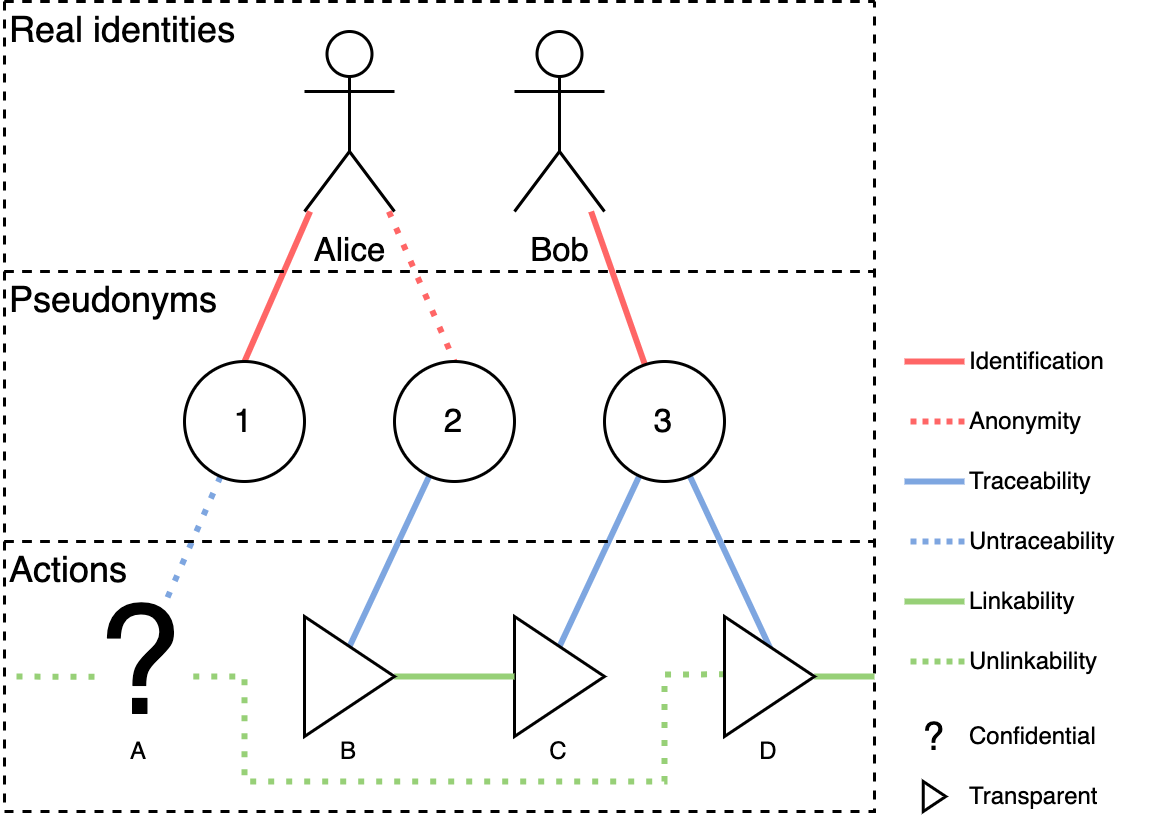
\includegraphics[width=9cm]{anonymity-diagram.png}
\centering
\caption{Let us assume the Alice to be the customer willing to keep her identity private (anonymous) and Bob be the public SP. Alice controls two addresses 1 and 2, the connection between her real identity and the first address was compromised, and therefore the identification is possible, the connection between the second pseudonym is still unknown therefore anonymous. Alice takes two actions; the first one from the compromised address and the second one from anonymous one. The first action is confidential; therefore even though the psudonym has been compromised the action can not be associated with the Alice. The second action is transparent, therefore the Alice's anonymity is maintained as long as the connection to the second pseudonym is concealed.}

\label{fig:anonymity-diagram1}
\end{figure}


The privacy-preserving blockchains are the ones that maintain anonymity via untraceability and (ideally) unlikability, not via assumption that the connection between an address and the real identity is concealed.   

Blockchains that natively support confidential transactions are
Monero~\cite{van2013cryptonote} (via Ring Signatures~\cite{cryptoeprint:2015:1098} and Bulletproofs~\cite{Bulletpr14, bunz2018bulletproofs}) and ZCash~\cite{sasson2014zerocash} (via zkSNARK~\cite{ben2013snarks}), Grin~\cite{fuchsbauer2019aggregate} (via Mimblewimble~\cite{httpsdow19}).

Overly techniques that achieve anonymity on top of non-privacy-preserving blockchains are: Ethereum's Tornado Cash\cite{pertsev2019tornado} (via zkSNARK~\cite{groth2016size} and MiMC~\cite{albrecht2016mimc}), Bitcoin's Wasabi\cite{WasabiWa56} (via CoinJoin \cite{CoinJoin41}).

\subsection{Payment for services}\label{payment-for-services}
Transactions between customers and SP have to be somehow pegged to prevent proving one payment for multiple transactions. In other
words, we need some way to uniquely link particular payment with the
the transaction paid for.

Depending on the cryptocurrency the link can be created in different
ways:

\begin{itemize}

\item
  separate address — each transaction derives a new address uniquely
  associating it with the transaction. Such addresses can be derived
  using Hierarchical Deterministic Wallets (BIP-32)~\cite{bipsbip089}.
\item
  memo — the payments are sent to one SP account but contain an extra
  field named ``memo'' which contains a random value generated by SP and
  included in $\mathrm{PoD}$. Each payment containing such value in the memo is
  considered to pay for the transaction in question. In case of a dispute,
  the connection can be disclosed by revealing the value in $\mathrm{PoD}$ and the payment's memo.
\end{itemize}

Both approaches have some advantages and disadvantages, but our protocol can abstract them away by treating them as some randomly generated unique number, often called \textit{nonce} (number once). How it is implemented depends on a particular blockchain.

In case of a dispute, there must be a way to prove to the justice that the customer has paid for the transaction. As the proof of transaction is trivial in transparent and trackable blockchains, it gets more complicated when it comes to anonymous blockchains. Monero allows proving and checking payments via dedicated API \cite{Howtopro46}. ZCash provides a mechanism called Payment Disclosure \cite{AnIntrod25}, which at the time of writing is still an experimental feature
\cite{paymentd11}.

\subsection{Storage network}\label{storage-network}
Once the SP finishes its service, he has to provide the result to the customer. The most natural approach would to be send the result via email of the dedicated platform. However, since the customer wants to stay anonymous, he doesn't want to expose his email address nor IP address. Moreover, in case of dispute, the SP should be able to prove that the result has been provided before the deadline.

One approach would be to post the result into a blockchain. Yet, storing data on a blockchain is very expensive. The most common workaround (\cite{shahid2020blockchain, wang2019auditable, chen2017improved, Usageide95}) is to publish the data to the IPFS \cite{benet2014ipfs}—a content addressable peer-to-peer storage network—and publish to a blockchain just a content identifier (cid) that uniquely points to the content stored on the IPFS.

We take the same approach. Once the SP creates the result, he encrypts it using the previously provided encryption key and uploads it to IPFS network.

To increase anonymity, the customer should use common techniques to hide its IP address; for example, use gateway, VPN, proxy, or onion routing.

\subsection{Separation of concerns}
We could use one blockchain to achieve all of these three roles: (i) anonymous payments; (ii) message board; (iii) storage network.

As the message board could be achieved by most of the blockchains, anonymous payments aren't so prevalent, and a provable storage network is a functionality of a few specialized blockchains.

Instead of searching for one blockchain that solves all the functionalities, we allow the protocol to use separate blockchains for each of the functionalities. In case a suitable blockchain arises, it can play more than one role.

At the time of writing, we see the following technologies that fulfill the requirements of each role:

\begin{enumerate}
\def\labelenumi{\arabic{enumi}.}

\item Anonymous payments: Monero \cite{van2013cryptonote}, ZCash
  \cite{sasson2014zerocash}, Grin \cite{fuchsbauer2019aggregate},
  Tornado Cash \cite{pertsev2019tornado}.
\item Message board: Stampery \cite{de2016stampery}, Proof of Existence
  \cite{proofofexistence} (Bitcoin blockchain), Chainpoint
  \cite{Chainpoi39} (Bitcoin blockchain), or any other blockchain that
  supports attaching extra data along the transaction.
\item Storage network: IPFS \cite{benet2014ipfs}, Filecoin
  \cite{benetfilecoin} (runs on top of IPFS), or Ethereum's
  Swarm\cite{swarmwhi49}.
\end{enumerate}

\section{The Protocol}\label{sec:protocol}

\subsection{Prerequisites}
We do not design our protocol with the assumption of usage particular technologies, instead, we define requirements that each party of the protocol must satisfy to make the whole system work together. The choice of the particular technology for each role is up to the developer.

\begin{itemize}
\item There exists common PKI infrastructure:
    \begin{itemize}
        \item The customer and the SP have their own key pairs consisting of secret key $\mathrm{sk}(\mathrm{party})$ and public key $\mathrm{pk}(\mathrm{party})$, where $\mathrm{party} \in \{\mathrm{C}, \mathrm{SP}\}$ is the customer or the service provider accordingly.
        \item Both the customer and the SP can create and verify digital signatures created by the customer $\mathrm{sig}_{\mathrm{sk}(\mathrm{C})}$ and the SP $\mathrm{sig}_{\mathrm{sk}(\mathrm{SP})}$.
        \item The SP's public key is publicly known.
    \end{itemize}
    
\item Both the customer and the SP:
    \begin{itemize}
        \item Uses common symmetric encryption $\mathrm{E}_\mathrm{key}(\cdot)$ and decryption $\mathrm{D}_\mathrm{key}(\cdot)$ operations.
    \end{itemize}

\item The SP:
    \begin{itemize}
        \item Accepts packages from unknown customers and give $\mathrm{PoD}$ in return.
        \item Accepts payments with anonymous cryptocurrencies as described in Section~\ref{payment-for-services}.
    \end{itemize}
    
\item Justice:
    \begin{itemize}
        \item Accepts as a evidence in dispute a $\mathrm{PoD}$, $\mathrm{PoP}$, and payment $\mathrm{attestation}$ as described in Section~\ref{proof-of-justice}.
    \end{itemize}

\item Anonymous payments:
    \begin{itemize}
        \item Supports anonymous, i.e., untraceable and (ideally) unlinkable transactions as specified in Section~\ref{sec:pseudo-anon}.
        \item Supports uniquely identifying transaction either via separate address, memo field, or other similar mechanisms as described in Section ~\ref{payment-for-services}. 
    \end{itemize}

\item Message board:
    \begin{itemize}
        \item Supports proofs as large as the size of $\mathrm{PoP}$, i.e., sum size of $\mathrm{cid}$, $\mathrm{nonce}$, and $\mathrm{sig}$.
    \end{itemize}

\item The storage network:
    \begin{itemize}
        \item Allows for uniquely content retrieval via $\mathrm{cid}$ (usually a hash of the content).
        \item Allows for anonymous content retrieval.
    \end{itemize}
\end{itemize}

\subsection{Messages}\label{messages}
In this section, we describe the messages exchanged between the parties of the protocol.

\noindent \textbf
{Package}\label{package} is a physical container prepared by the customer encompassing all $\mathrm{materials}$ required by the SP to provide the service, and an encryption $\mathrm{key}$ used to encrypt the result published on the storage network.

$$\mathrm{pkg} \equiv (\mathrm{materials}, \mathrm{key})$$

where:

\begin{itemize}

\item $\mathrm{materials}$ - are the materials required to provide the service. For example samples of urine, blood, stool, saliva; legal documents, CDs, emails, photos, bank statements, or any other kind of evidence depending on the service.
\item $\mathrm{key}$ - symmetric key used to encrypt and decrypt the result.
\end{itemize}

\noindent \textbf
{Proof of delivery ($\mathrm{PoD}$)}\label{proof-of-delivery} is a  confirmation issued by the SP to the customer that proves that the customer has delivered to the SP a complete (according to the SP requirements) package, and the SP accepted it.

It is also an agreement between the customer and the SP, as it includes agreed upfront deadlines of actions in the protocol.

We assume the $\mathrm{PoD}$ to be a QR code printed on a paper receipt, but any other form that guarantees integrity, authenticity, and non-repudiation can be used instead. 

The ($\mathrm{PoD}$ can be then used as evidence in case of a dispute.

$$\mathrm{PoD} \equiv (\mathrm{T}_\mathrm{issue}, \mathrm{T}_\mathrm{pay}, \mathrm{T}_\mathrm{provide}, \mathrm{nonce}, \mathrm{sig}_\mathrm{SP})$$

where:

\begin{itemize}

\item $\mathrm{T}_\mathrm{issue}$ - time at which the PoD is issued.
\item
  $\mathrm{T}_\mathrm{pay}$ - deadline to pay for the transaction.
\item
  $\mathrm{T}_\mathrm{provide}$ - deadline to provide a result of the service.
\item $\mathrm{nonce}$ - randomly generated number uniquely identifying the transaction.
\item $\mathrm{sig}_\mathrm{SP}$ - the SP's signature guaranteeing non-repudiation.
\end{itemize}

also:
\(\mathrm{T}_\mathrm{issue} < \mathrm{T}_\mathrm{pay} < \mathrm{T}_\mathrm{provide}\)

\noindent \textbf
{Proof of provision ($\mathrm{PoP}$)}\label{proof-of-provision} is proof that the SP published the result at a certain time. It defends the SP in case the customer unjustly starts a dispute after the result has been published. The connection between $\mathrm{PoP}$ and the result is made by the content identifier ($(\mathrm{cid}$) that uniquely identify the result (it is some kind of a hash of the result) such that the result can not be forged after the $\mathrm{PoP}$ has been published.

The $\mathrm{PoP}$ is a digital construction published by the SP on the message board.

\[\mathrm{PoP} \equiv (\mathrm{cid}, \mathrm{nonce}, \mathrm{sig}_\mathrm{SP})\]

where:

\begin{itemize}

\item
  \(\mathrm{cid}\) - content identifier as specified in ~\ref{storage-network}.
\item
  \(\mathrm{nonce}\) - the value uniquely identifying the transaction previously generated in $\mathrm{PoD}$.
\item
  \(\mathrm{sig}_\mathrm{SP}\) - the SP's signature guaranteeing authentication.
\end{itemize}

\noindent \textbf
{Payment attestation}\label{payment-attestation}
proves that the customer did the payment. Since the
evidence depends on the particular blockchain (see Section ~\ref{payment-for-services}). We refer to them symbolically as
\(attestation\).

\noindent \textbf
{Result}\label{results} is assumed to be document in PDF format, but any other format is allowed as long as it can be binary encoded and uploaded to IPFS. We refer to it symbolically as $result$.

\noindent \textbf
{Content Identifier (cid)}\label{content-identifier-cid}  is a term coined by IPFS
\cite{Contenta59}  
. However, since our protocol does not depend on
this particular implementation of the storage network, we let the cid be any
other identifier that securely and uniquely points to the content.

\subsection{Protocol description}\label{protocol-description}

In this section, we describe each step of the protocol. The steps are
shown in the Figure ~\ref{fig:protocol-diagram}.

\begin{figure}[h!]
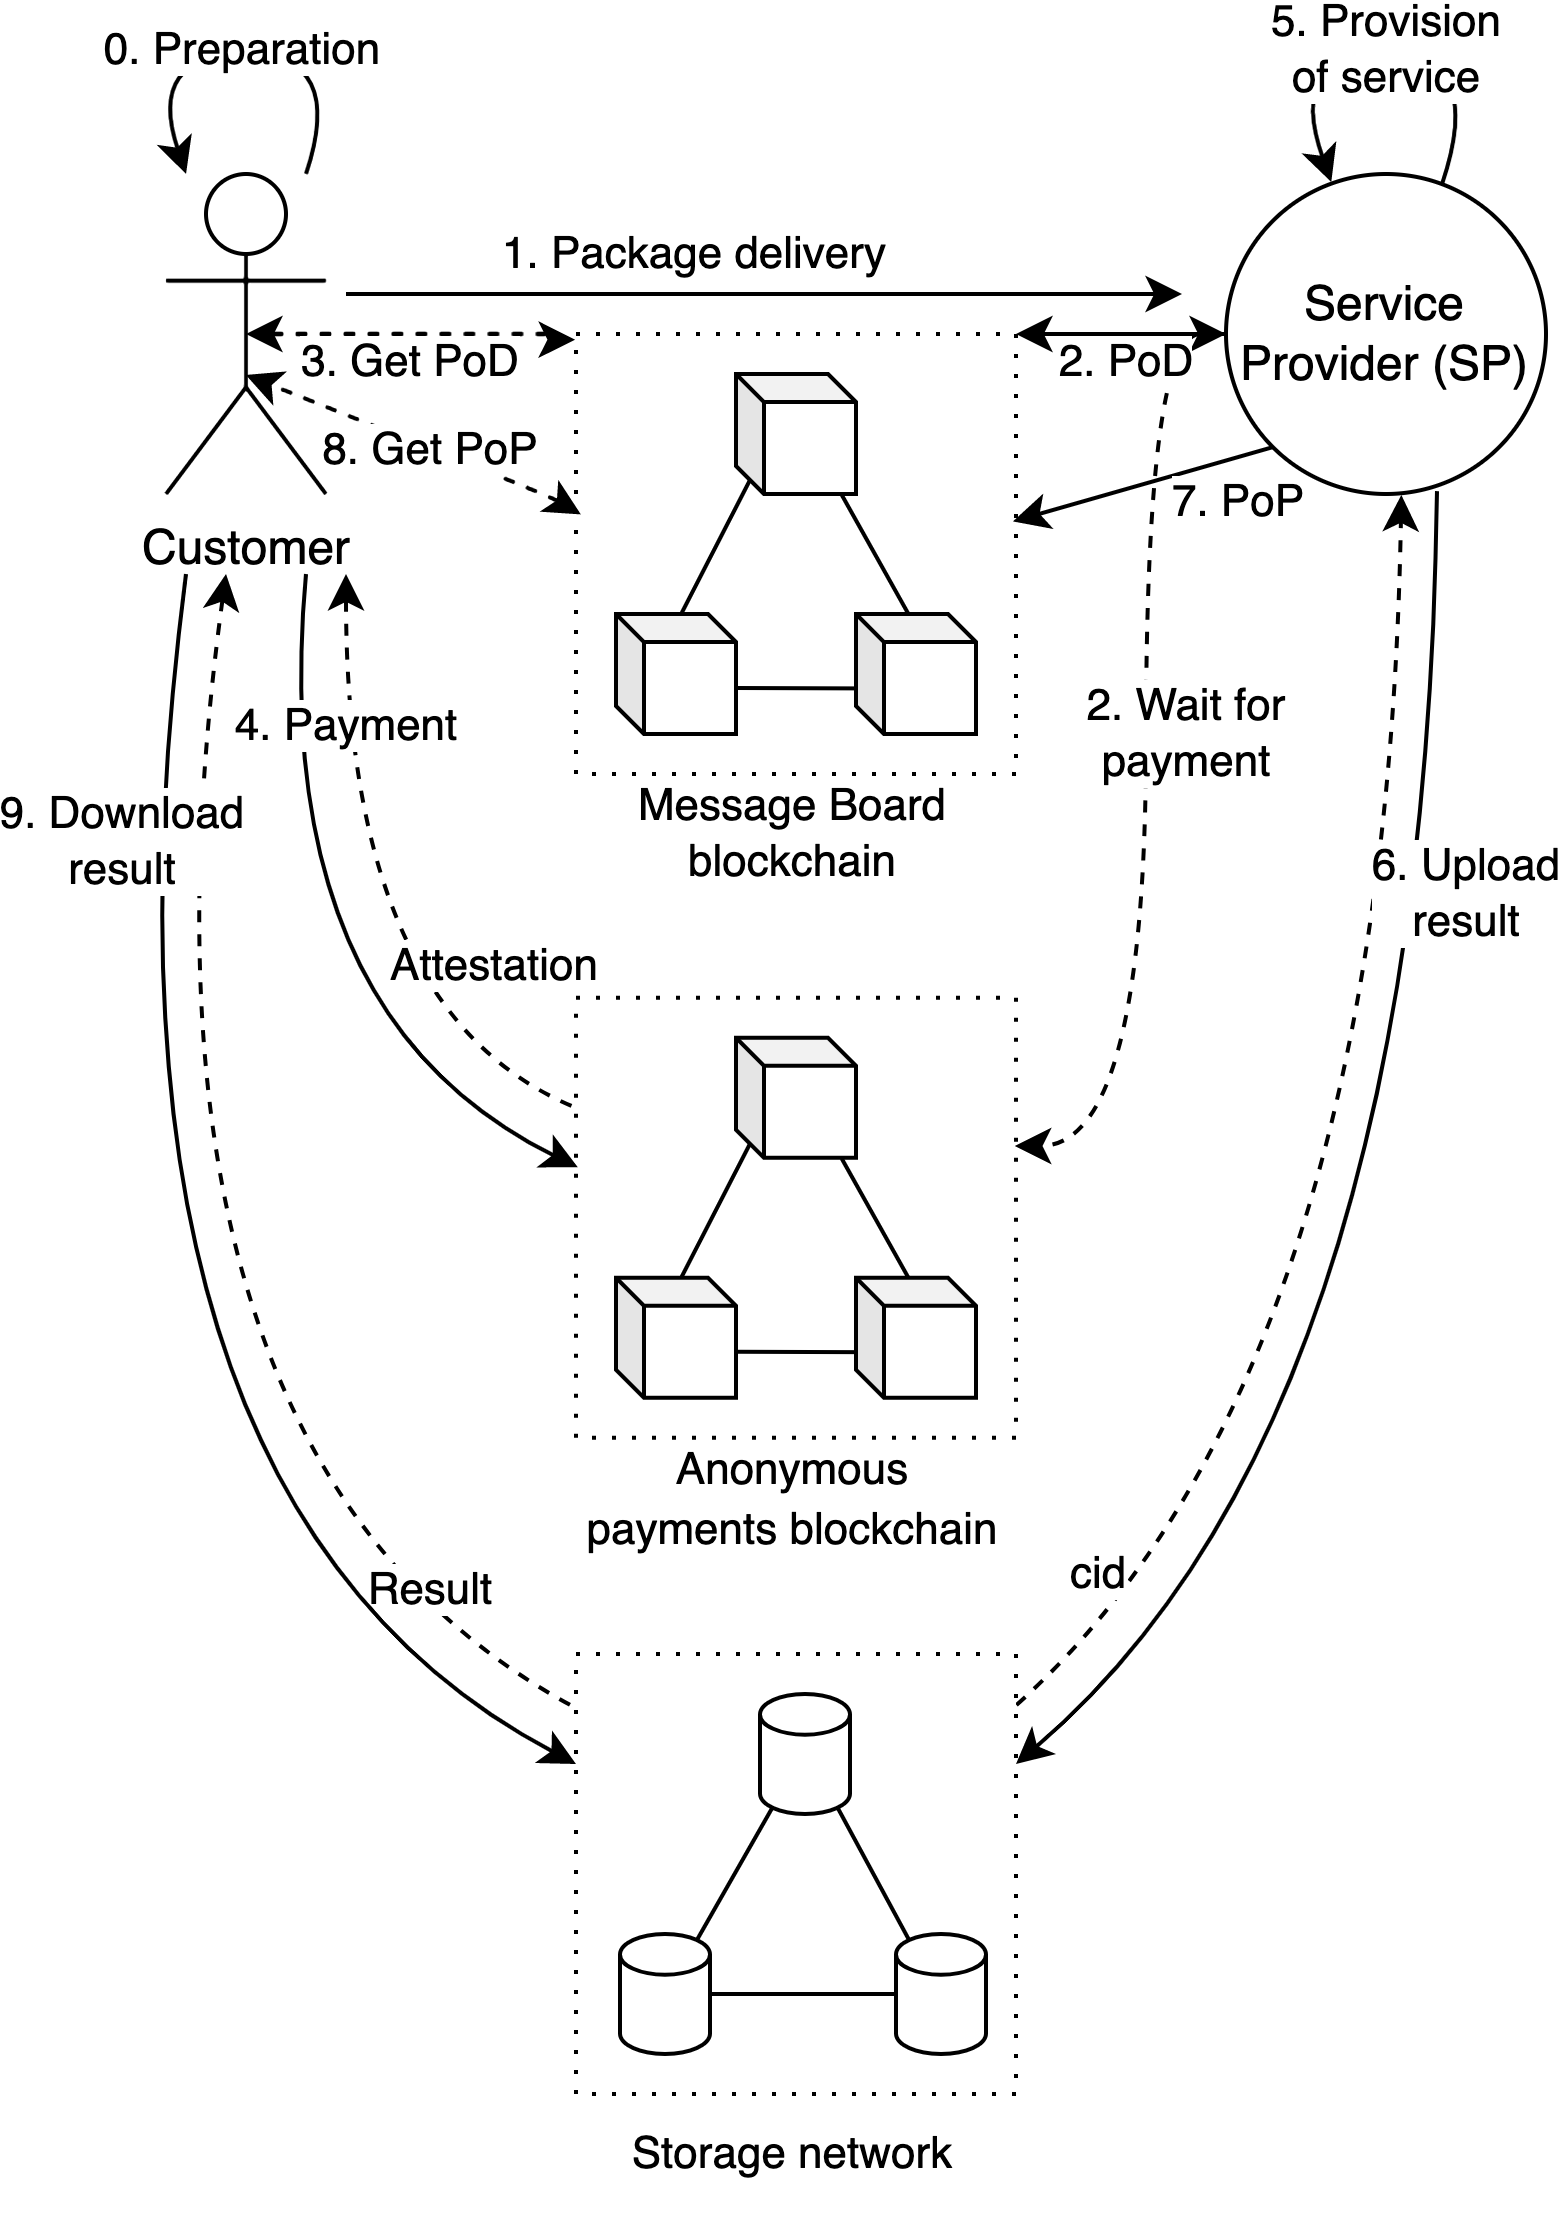
\includegraphics[width=9cm]{anonser-protocol.png}
\centering
\caption{Messages exchanged in protocol.}
\label{fig:protocol-diagram}
\end{figure}

\noindent \textbf
{Step 0.  Preparation}\label{step-0-preparation}

The customer collects all the $\mathrm{materials}$ required by the SP, generates an encryption $\mathrm{key}$ prints it on a paper as a QR code, and packs them together into a package $\mathrm{pkg}$.

Symbolically: 
$
\mathrm{pkg} \gets (\mathrm{materials}, \mathrm{key})
$

\noindent \textbf
{Step 1. Package delivery}\label{step-1-package-delivery}

They protocol starts once the customer delivers package $\mathrm{pkg}$ and the SP accepts its content. In return, the SP issue a $\mathrm{PoD}$ with agreed upfront payment deadline $\mathrm{T}_\mathrm{pay}$, service provision deadline $\mathrm{T}_\mathrm{provide}$ and current time $\mathrm{T}_\mathrm{issue}$. Also, the $\mathrm{PoD}$ consist of randomly generated unique number $\mathrm{nonce}$, which will allow associating all actions related to the transaction throughout the protocol. Finally, the digital signature $\mathrm{sig}_{\mathrm{sk}(\mathrm{SP})}$ on the $\mathrm{PoD}$ created with the SP's secret key $\mathrm{sk}(\mathrm{SP})$ guarantee non-repudiation.

We assume this step to be fully physical, that is, $\mathrm{pkg}$ consists of physical materials, $\mathrm{PoD}$ is in a form of e.g., QR code printed on a paper receipt. 

$\mathrm{PoD}$ could be published on a message board (similarly to $\mathrm{PoP}$); however, since the $\mathrm{pkg}$ is delivered personally or via a trusted person, the confirmation can be issued in person as well. If we would like to hire a courier to deliver our $\mathrm{pkg}$, then the $\mathrm{PoD}$ would have to be published on the message board (further extension to the anonymous delivery system is discussed in Section \ref{sec:future-work}).

Symbolically: 
$
\mathrm{PoD} \gets \mathrm{delivery}(\mathrm{pkg})
$

$
(\mathrm{T}_\mathrm{issue}, \mathrm{T}_\mathrm{pay}, \mathrm{T}_\mathrm{provide}, \mathrm{nonce}, \mathrm{sig}_{\mathrm{sk}(\mathrm{SP})}) \equiv \mathrm{PoD}
$


\noindent \textbf
{Step 2. Payment}\label{step-2-payment}

Having the PoD issued, the SP can not reject receiving the package. At this point the
customer should pay for the transaction with an agreed upfront cryptocurrency system (see Section~\ref{payment-for-services}).

In return, the customer receives the $\mathrm{attestation}$ that should be disclosed in case of a dispute.

Symbolically: 
$
\mathrm{attestation} \gets \mathrm{payment}(\mathrm{nonce}, \mathrm{sig}_{\mathrm{sk}(\mathrm{C})})
$

\noindent \textbf
{Step 3. Provision of service}\label{step-3-provision-of-service} 
Once the transaction is paid the SP starts the provision of service.

Symbolically: 
$
\mathrm{result} \gets \mathrm{provision}(\mathrm{materials})
$

\noindent \textbf
{Step 4. Upload result }\label{step-4-results-upload}

After the service is finished, some result should be created. Next, the result is encrypted using encryption symmetric $\mathrm{key}$ provided in the first step.

The encrypted result is then uploaded on the content addressable network such as IPFS. In return the content identifier (cid) is created.

Symbolically: 
$
\mathrm{cid} \gets \mathrm{upload}(E_{\mathrm{key}}(\mathrm{result}))
$

\noindent \textbf
{Step 5. Proof of provision publication}\label{step-5-proof-of-provision-publication}

When the result is published, the SP performs proof of provision by publishing $\mathrm{cid}$ along with $\mathrm{nonce}$ and signature $\mathrm{sig}_\mathrm{SP}$.

Symbolically: 
$
\mathrm{PoP} \equiv (\mathrm{cid}, \mathrm{nonce}, \mathrm{sig}_{\mathrm{sk}(\mathrm{SP})})
$

$
\mathrm{publish}(\mathrm{PoP})
$

\noindent \textbf
{Step 6. Proof-of-provision notification}\label{step-6-proof-of-provision-notification}

After delivering the package and paying for the transaction the customer subscribes to the message board and waits until the SP publishes the proof of provision. The subscription is for the SP public key $\mathrm{pk}(\mathrm{SP}$ and transaction's $\mathrm{nonce}$.

Symbolically: 
$
\mathrm{cid} \gets \mathrm{subscribe}(\mathrm{pk}(\mathrm{SP}), \mathrm{nonce})
$

\noindent \textbf
{Step 7. Result download}\label{step-7-results-download} 
Having the $\mathrm{cid}$, the customer downloads and decrypts the $\mathrm{result}$.

Symbolically: 
$
\mathrm{result} \gets \mathrm{D}_{\mathrm{key}}(\mathrm{download}(\mathrm{cid}))
$


\section{Fairness analysis}\label{sec:fairness-analysis}

We analyze the fairness of the protocol by representing it as an interactive non-cooperative game.

\subsection{Model}\label{model}
We consider three positions:

\begin{itemize}
\item
  Neutral position (•): when a party hasn't spent nor gained anything of significant value (money, time, effort). For example, at the beginning of the protocol.
\item
  Disadvantaged position (-): when a party has put a significant value without receiving an equivalent. For example, paid for a service in advance.
\item
  Advantaged position (+): when a party would benefit if the transaction would halt at that step. For example, the SP has received payment before service provision.
\end{itemize}

There are many actions that each party can take, but we group them into two categories:

\begin{enumerate}
\def\labelenumi{\arabic{enumi}.}

\item
  Normal: taking the action prescribed by the protocol.
\item
  Abnormal: everything that deviates from the designed steps of the protocol. For example, sending an arbitrary message, skipping some step, repeating step, timing out.
\end{enumerate}

Moreover, at any step of the protocol, the customer can start a dispute; therefore, another dimension with two positions has to be considered:

\begin{enumerate}
\def\labelenumi{\arabic{enumi}.}

\item
  Agree: the customer agrees with the action and therefore does not start a dispute.
\item
  Start a dispute: the customer does not agree with the action and therefore starts a dispute.
\end{enumerate}

As a result, in our analysis we have to consider four different outcomes for each party of the protocol:

\begin{itemize}

\item
  $\sigma_\mathrm{n}$: after following the protocol when the other party acted normally.
\item
  $\sigma_\mathrm{d}$: after a settled dispute when the other party acted normally.
\item
  $\sigma_\overline{n}$: after not starting a dispute despite the other party has acted abnormally.
\item
  $\sigma_\overline{d}$: after a settled dispute when the other party has acted abnormally.
\end{itemize}

The protocol terminates after the last step, after starting a dispute, or after a party hasn't completed its designated action in time. Therefore, all positions except $\sigma_\mathrm{n}$ are termination positions.

Because the customer is anonymous the SP can not start a dispute---there is no means to identify the customer. To mitigate the issue, we designed the protocol so that the SP who follows the protocol is always in an advantageous position, therefore he has no reason to start a dispute. The customer on the other hand can start a dispute at any time of the protocol, but only the actual misbehavior of the SP makes him win the case.

\begin{definition}[Fairness] \label{fairness}
A protocol achieve fariness iff 
\begin{equation*}
\begin{split}
\forall_{party \in parties}\forall_{\mathrm{step} \in \mathrm{steps}} &\mathrm{can\ move}\\
&\mathrm{to\ the\ non\ disadvantaged\ position} 
\end{split}
\end{equation*}

\end{definition}


\subsection{Assumptions}\label{assumptions}

Below  we listed
assumptions we took
for the analysis purpose.  

\begin{itemize}

\item
  Both parties start from a neutral position (•).
\item
  Both parties, by completing a transaction, end up in advantaged positions (+). In other words, they have intrinsic motivation to initialize and complete the transaction.
\item
  We assume the steps of the protocol to be atomic, there are no intermediate steps.
\item
  Repeating the first step starts a new transaction. Repeating any other step is considered abnormal and gets ignored. For example, paying for the invoice twice does not cause any effect on the curse of the protocol.
\item
  Once published, the result is available to the customer in the content storage. The idea of guaranteeing it cryptographically is discussed in Section~\ref{sec:future-work}.
  
  
\item
  The protocol can go only forward, there is no way of reverting any action.
\item
  Losing the dispute leads to a punishment that is greater than any reward, which leads to a disadvantaged position (-). Hence, the rational customer won't start a dispute that he is not sure to win.
\item
  Winning the dispute leads to a neutral position (•).
\item
  Both the customer and the SP are rational (selfish). They always prefer to go from worst position to better position, but also risk temporary worst position in favor of a later better position iff it's assured that they won't be stuck in the worst position.
\end{itemize}

\subsection{Steps}\label{steps}

Figure~\ref{fig:positions} 
shows the positions of each party after each possible action taken.

\begin{figure}[h!]
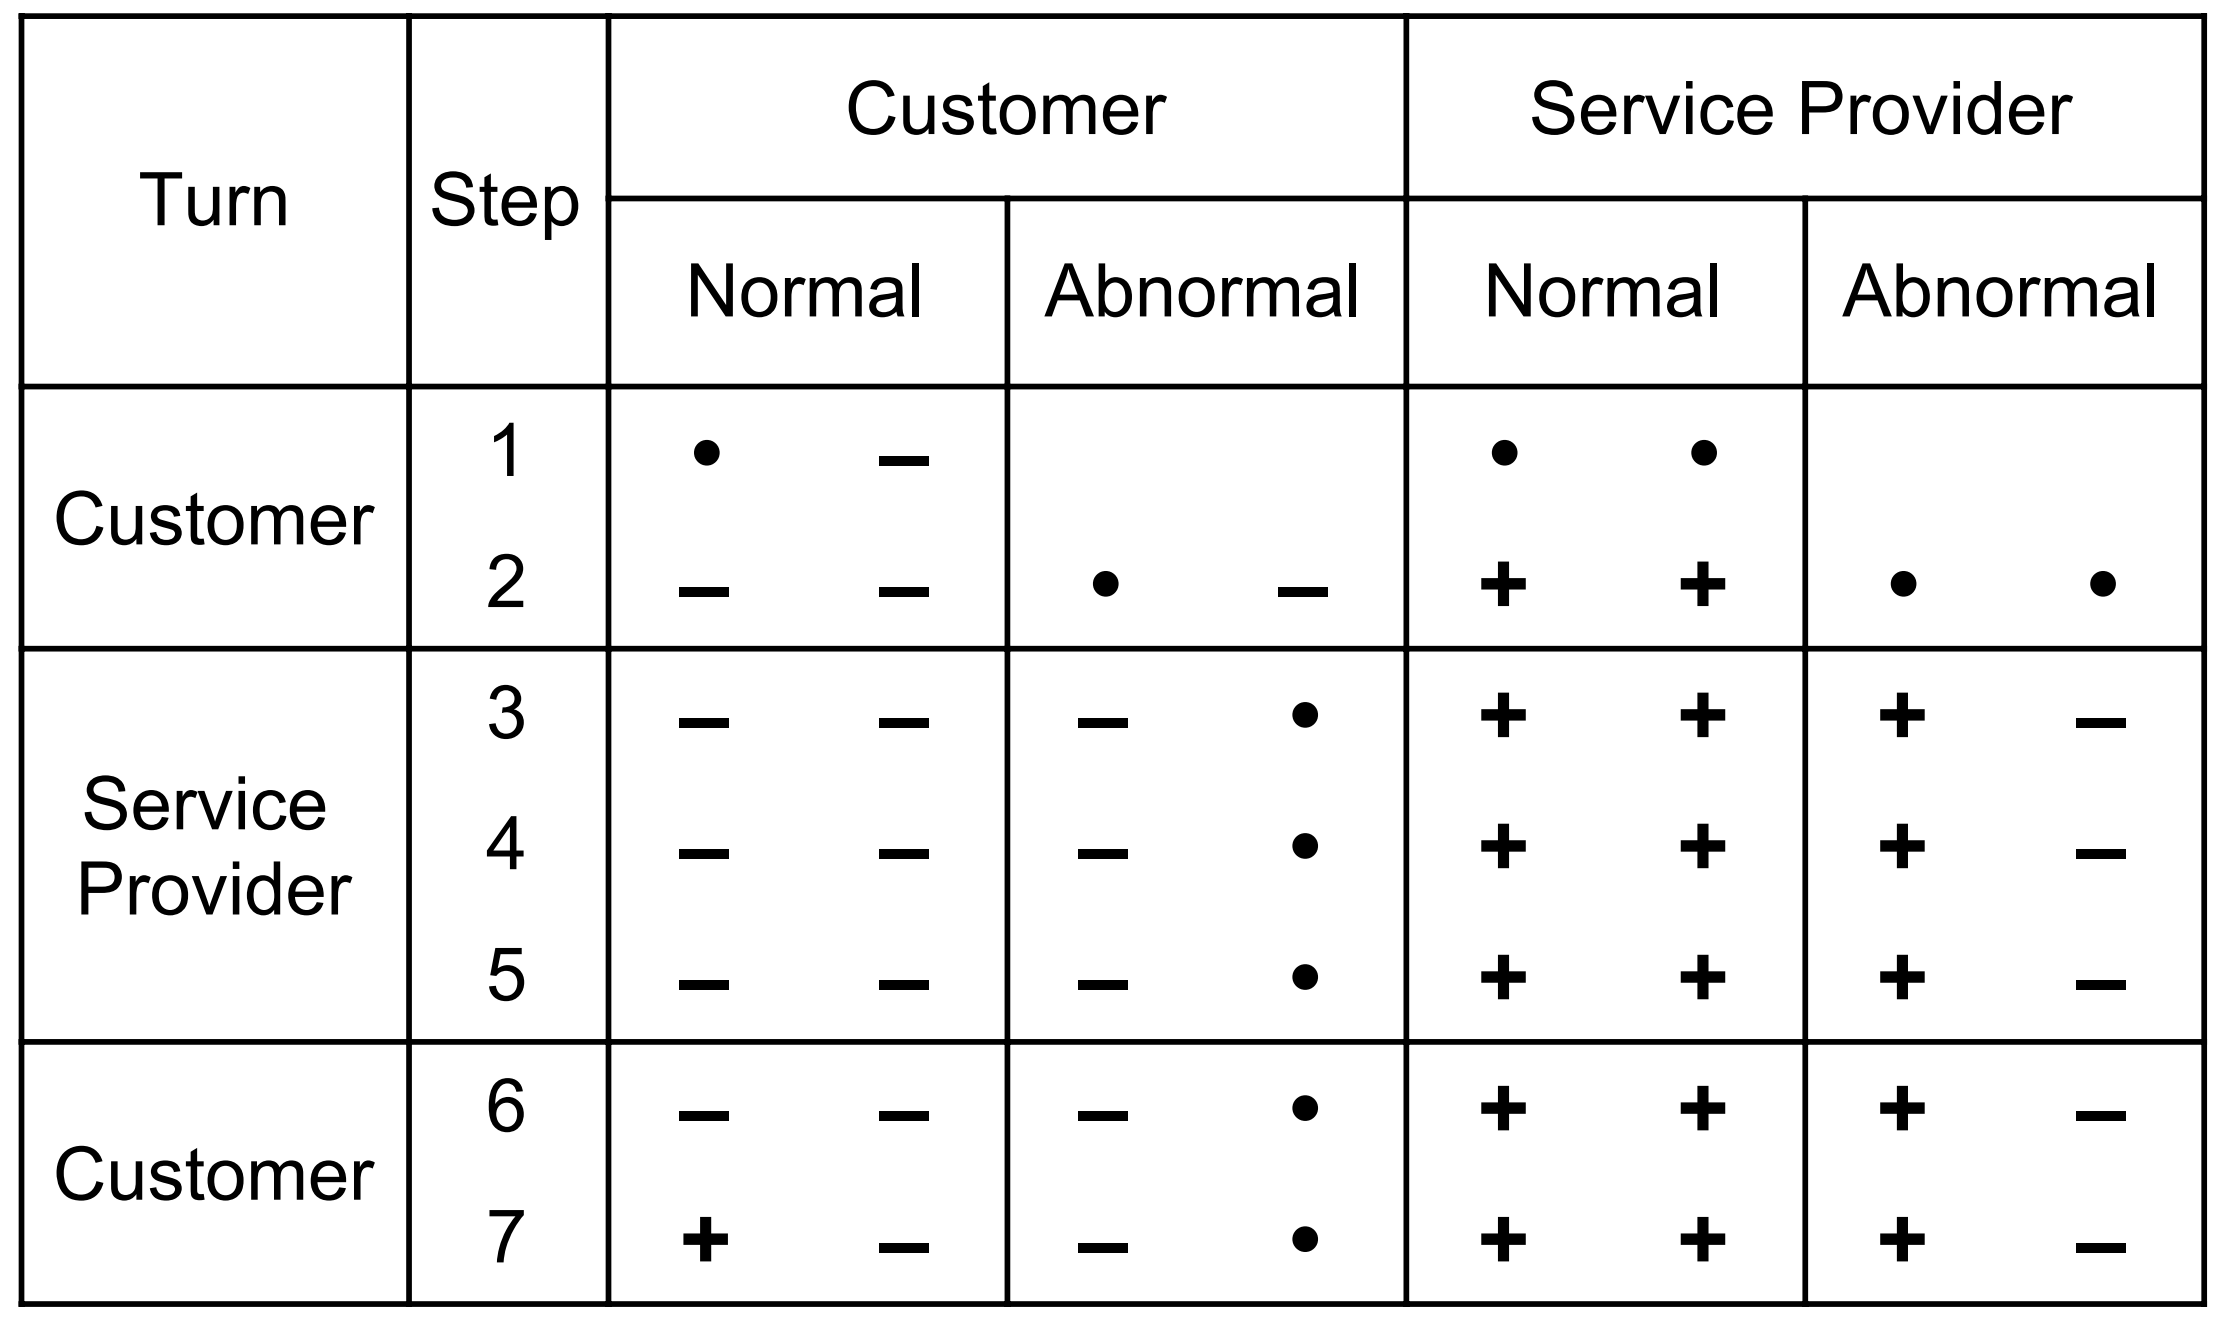
\includegraphics[width=9cm]{formal-table-of-positions.png}
\centering
\caption{Positions after each step of protocol}
\label{fig:positions}
\end{figure}


Below we describe each step and rationale of the outcome position.


\noindent \textbf
{Step 1. Customer turn: deliver package}\label{step-1-deliver-package}

Customer has delivered the package:

\begin{itemize}
\item
  Agreeable path:

  \begin{itemize}
  
  \item
    \(\sigma_{1, c, \mathrm{n}} = \sbullet\), the customer has risked its
    materials but has not paid anything, so we assume he is in neutral
    position. One would argue that the customer has put effort of
    delivering the materials to the SP, or that the sample is valuable.
    We assume that the sample without personal information is useless
    and the effort to deliver the package is negligible.
  \item
    \(\sigma_{1, s, \mathrm{n}} = \sbullet\), the SP is in the neutral position as he didn't put any effort to hence the package, also the package hasn't any value to the SP.
  \end{itemize}
\item
  Starting a dispute:

  \begin{itemize}
  
  \item
    \(\sigma_{1, c, \mathrm{d}} = -\), the customer loses the case as the SP has still an opportunity to publish proof-of-provision within the timeframe.
  \item
    \(\sigma_{1, s, \mathrm{d}} = \sbullet\), the SP win the case for the same reason.
  \end{itemize}
\end{itemize}

Fairness:

\begin{itemize}

\item
  The customer can follow the protocol and move to a non-disadvantaged
  position \(\sigma_{1, c, \mathrm{n}} = \sbullet\).
\item
  The SP can do nothing and end up in a non-disadvantaged position
  \(\sigma_{1, s, \mathrm{n}} = \sbullet \) or
  \(\sigma_{1, s, \mathrm{d}} = \sbullet \).
\end{itemize}

\noindent \textbf
{Step 2. Customer turn: pay for invoice}\label{step-2-pay-for-invoice}

Customer has paid the invoice:

\begin{itemize}
\item
  Following protocol:
  \begin{itemize}
  \item
    \(\sigma_{2, c, \mathrm{n}} = -\), the customer has spent his funds but hasn't received the result.
  \item
    \(\sigma_{2, s, \mathrm{n}} = +\), the SP has received the payment but hasn't spent his resources yet.
  \end{itemize}
\item
  Starting a dispute:

  \begin{itemize}
  \item
    \(\sigma_{2, c, \mathrm{d}} = -\), the customer loses the case as the SP has still an opportunity to publish proof-of-provision before the deadline.
  \item
    \(\sigma_{2, s, \mathrm{d}} = +\), the SP win the case for the same reason.
  \end{itemize}
\end{itemize}

Customer has timeouted, then:

\begin{itemize}
\item
  Following protocol:
  \begin{itemize}
  \item
    \(\sigma_{2, c, \overline{\mathrm{n}}} = \sbullet\), the customer ends up in a neutral position, since he didn't spend his funds.
  \item
    \(\sigma_{2, s, \overline{\mathrm{n}}} = \sbullet\), the SP ends up in a neutral position as he didn't receive the payment, nor spent his resources.
  \end{itemize}
\item
  Starting a dispute:

  \begin{itemize}
  
  \item
    \(\sigma_{2, c, \overline{\mathrm{d}}} = -\), the customer loses the case as he can not prove the payment before the time limit.
  \item
    \(\sigma_{2, s, \overline{\mathrm{d}}} = \sbullet\), the SP is not charged to justice due to a lack of proof.
  \end{itemize}
\end{itemize}

Fairness:

\begin{itemize}

\item
  The customer can move the protocol forward to step 3, where if the
  SP follows the protocol then the customer can push the protocol forward
  up to the last termination step \(\sigma_{7, c, \mathrm{n}} = +\),
  otherwise if at any step the SP does not follow the protocol the
  customer can start a dispute which terminates the protocol at
  non-disadvantaged position, i.e.,
  \(\sigma_{3, c, \overline{\mathrm{d}}} = \sbullet\),
  \(\sigma_{4, c, \overline{\mathrm{d}}} = \sbullet\),
  \(\sigma_{5, c, \overline{\mathrm{d}}} = \sbullet\).
\item
  The SP can do nothing and end up in non-disadvantaged position
  \(\sigma_{2, s, \mathrm{n}} = +\), \(\sigma_{2, s, \mathrm{d}} = +\),
  \(\sigma_{2, s, \overline{\mathrm{n}}} = \sbullet\),
  \(\sigma_{2, s, \overline{\mathrm{d}}} = \sbullet\).
\end{itemize}

\noindent \textbf
{Step 3. SP turn: provision of service}\label{step-3-provision-of-service}

The SP has done the provision of service:

\begin{itemize}
\item
  Following protocol:

  \begin{itemize}
  
  \item
    \(\sigma_{3, c, \mathrm{n}} = -\), the customer hasn't received the
    result so he remains in a disadvantaged position.
  \item
    \(\sigma_{3, s, \mathrm{n}} = +\), the SP has fulfilled the contract
    on time.
  \end{itemize}
\item
  Starting a dispute:

  \begin{itemize}
  
  \item
    \(\sigma_{3, c, \mathrm{d}} = -\), the customer lose the case as the
    SP has still the opportunity to publish proof-of-provision within
    timeframe.
  \item
    \(\sigma_{3, s, \mathrm{d}} = +\), the SP win the case for the same
    reason.
  \end{itemize}
\end{itemize}

SP has timeouted, then:

\begin{itemize}
\item
  Following protocol:

  \begin{itemize}
  
  \item
    \(\sigma_{3, c, \overline{\mathrm{n}}} = -\), the customer ends up in a disadvantaged position.
  \item
    \(\sigma_{3, s, \overline{\mathrm{n}}} = +\), the SP ends up in a
    advantaged position as he received the payment.
  \end{itemize}
\item
  Starting a dispute:

  \begin{itemize}
  
  \item
    \(\sigma_{3, c, \overline{\mathrm{d}}} = •\), the customer wins the case and ends up in a neutral position.
  \item
    \(\sigma_{3, s, \overline{\mathrm{d}}} = -\), the SP loses the case
    and end up in a disadvantaged position.
  \end{itemize}
\end{itemize}

Fairness:

\begin{itemize}

\item
  The customer can do nothing if the SP follows the protocol, which will
  ultimately put him in an advantaged position
  \(\sigma_{7, c, \mathrm{n}} = +\), or in case of the SP not following
  the protocol, the customer can start a dispute and terminate in a
  non-disadvantaged position
  \(\sigma_{3, c, \overline{\mathrm{d}}} = •\).
\item
  The SP can follow the protocol and move to a non-disadvantaged
  position \(\sigma_{3, s, \mathrm{n}} = +\), or not follow the protocol
  and also end up at a non-disadvantaged position
  \(\sigma_{3, s, \overline{\mathrm{n}}} = +\), but the second option
  puts him at risk of terminating the protocol at
  \(\sigma_{3, s, \overline{\mathrm{n}}} = +\), if the customer is
  rational and starts a dispute.
\end{itemize}

\noindent \textbf
{Step 4. SP turn: upload result}\label{step-4-publication-of-results}

SP has uploaded the result on time:

\begin{itemize}
\item
  Following protocol:

  \begin{itemize}
  
  \item
    \(\sigma_{4, c, \mathrm{n}} = -\), the customer hasn't received the result so he remains in disadvantaged position.
  \item
    \(\sigma_{4, s, \mathrm{n}} = +\), the SP has fulfilled the contract on time.
  \end{itemize}
\item
  Starting a dispute:

  \begin{itemize}
  
  \item
    \(\sigma_{4, c, \mathrm{d}} = -\), the customer lose the case as the
    SP has still opportunity to publish proof-of-provision within
    timeframe.
  \item
    \(\sigma_{4, s, \mathrm{d}} = +\), the SP win the case for the same
    reason.
  \end{itemize}
\end{itemize}

SP has timeouted, then:

\begin{itemize}
\item
  Following protocol:

  \begin{itemize}
  
  \item
    \(\sigma_{4, c, \overline{\mathrm{n}}} = -\), the customer ends up in
    disadvantaged position.
  \item
    \(\sigma_{4, s, \overline{\mathrm{n}}} = +\), the SP ends up in
    advantaged position as he received the payment.
  \end{itemize}
\item
  Starting a dispute:

  \begin{itemize}
  
  \item
    \(\sigma_{4, c, \overline{\mathrm{d}}} = •\), the customer wins the
    case and end up in neutral position.
  \item
    \(\sigma_{4, s, \overline{\mathrm{d}}} = -\), the SP loses the case
    and end up in a disadvantaged position.
  \end{itemize}
\end{itemize}

Fairness:

\begin{itemize}

\item
  The customer can do nothing if the SP follows the protocol, which will
  ultimately put him in an advantaged position
  \(\sigma_{7, c, \mathrm{n}} = +\), or in case of the SP not following
  the protocol, the customer can start a dispute and terminate in
  non-disadvantaged position
  \(\sigma_{4, c, \overline{\mathrm{d}}} = \sbullet\).
\item
  The SP can follow the protocol and move to the non-disadvantaged
  position \(\sigma_{4, s, \mathrm{n}} = +\), or not follow the protocol
  and also end up at non-disadvantaged position
  \(\sigma_{4, s, \overline{\mathrm{n}}} = +\), but the second option
  puts him at risk of terminating the protocol at
  \(\sigma_{4, s, \overline{\mathrm{n}}} = +\), if the customer is
  rational and starts a dispute.
\end{itemize}

\noindent \textbf
{Step 5. SP turn: publication of proof-of-provision}\label{step-5-publication-of-proof-of-provision}

The SP has published proof of provision on time:

\begin{itemize}
\item
  Following protocol:

  \begin{itemize}
  
  \item
    \(\sigma_{5, c, \mathrm{n}} = -\) the customer hasn't received the
    result. Therefore, he remains in a disadvantaged position.
  \item
    \(\sigma_{5, s, \mathrm{n}} = +\) the SP has fulfilled the contract
    on time.
  \end{itemize}
\item
  Starting a dispute:

  \begin{itemize}
  
  \item
    \(\sigma_{5, c, \mathrm{d}} = -\) the customer lose the case as the
    SP can prove the publication of proof-of-provision.
  \item
    \(\sigma_{5, s, \mathrm{d}} = +\) the SP win the case as the SP can
    prove the publication of proof-of-provision.
  \end{itemize}
\end{itemize}

SP has timeouted, then:

\begin{itemize}
\item
  Following protocol:

  \begin{itemize}
  
  \item
    \(\sigma_{5, c, \overline{\mathrm{n}}} = -\) the customer ends up in a disadvantaged position.
  \item
    \(\sigma_{5, s, \overline{\mathrm{n}}} = +\) the SP ends up in
    an advantaged position as he received the payment.
  \end{itemize}
\item
  Starting a dispute:

  \begin{itemize}
  
  \item
    \(\sigma_{5, c, \overline{\mathrm{d}}} = •\) the customer wins the
    case and end up in a neutral position.
  \item
    \(\sigma_{5, s, \overline{\mathrm{d}}} = -\) the SP loses the case
    and end up in a disadvantaged position.
  \end{itemize}
\end{itemize}

Fairness:

\begin{itemize}

\item
  The customer can do nothing if the SP follows the protocol because it
  will ultimately put him in an advantaged position
  \(\sigma_{7, c, \mathrm{n}} = +\), otherwise, in case of the SP not
  following the protocol, the customer can start a dispute and terminate
  in non-disadvantaged position
  \(\sigma_{5, c, \overline{\mathrm{d}}} = •\).
\item
  The SP can follow the protocol and move to the non-disadvantaged
  position \(\sigma_{5, s, \mathrm{n}} = +\), or not follow the protocol
  and also end up at non-disadvantaged position
  \(\sigma_{5, s, \overline{\mathrm{n}}} = +\), but the second option
  puts him at risk of terminating the protocol at
  \(\sigma_{5, s, \overline{\mathrm{n}}} = +\), if the customer is
  rational and starts a dispute.
\end{itemize}


\noindent \textbf
{Step 6. customer turn: pull proof of provision}\label{step-6-pull-proof-of-provision}

SP has uploaded the result on time, then:

\begin{itemize}
\item
  Follows the protocol:

  \begin{itemize}
  
  \item
    \(\sigma_{6, c, \mathrm{n}} = -\) the customer gets hash of the
    result but not the result yet.
  \item
    \(\sigma_{6, s, \mathrm{n}} = +\) the SP position hasn't changed.
  \end{itemize}
\item
  Starts a dispute:

  \begin{itemize}
  
  \item
    \(\sigma_{6, c, \mathrm{d}} = -\) the customer lose the case as the
    SP can prove the publication of proof-of-provision.
  \item
    \(\sigma_{6, s, \mathrm{d}} = +\) the SP win the case as the SP can
    prove the publication of proof-of-provision.
  \end{itemize}
\end{itemize}

Customer has timeouted, then:

\begin{itemize}
\item
  Follows the protocol:

  \begin{itemize}
  
  \item
    \(\sigma_{6, c, \overline{\mathrm{n}}} = -\) the customer ends up in
    disadvantaged position.
  \item
    \(\sigma_{6, s, \overline{\mathrm{n}}} = +\) the SP ends up in
    advantaged position as he received the payment but didn't spend his
    resources.
  \end{itemize}
\item
  Starts a dispute:

  \begin{itemize}
  
  \item
    \(\sigma_{6, c, \overline{\mathrm{d}}} = •\) the customer wins the
    case and end up in a neutral position.
  \item
    \(\sigma_{6, s, \overline{\mathrm{d}}} = -\) the SP loses the case
    and end up in a disadvantaged position.
  \end{itemize}
\end{itemize}

Fairness:

\begin{itemize}

\item
  The customer can follow the protocol to the position
  \(\sigma_{6, c, \mathrm{n}} = -\), which let's him move the protocol
  to a non-disadvantaged termination position
  \(\sigma_{7, c, \mathrm{n}} = +\), or in case the SP haven't followed
  the protocol start a dispute and win the case
  \(\sigma_{6, c, \overline{\mathrm{d}}} = \sbullet\).
\item
  The SP can do nothing and end up in a non-disadvantaged position
  \(\sigma_{6, s, \mathrm{n}} = +\), or
  \(\sigma_{6, s, \overline{\mathrm{n}}} = +\).
\end{itemize}

\noindent \textbf
{Step 7. Customer turn: result download}\label{step-7-retrieval-of-results}

SP has published the \textbf{correct} result on time:

\begin{itemize}
\item
  Following protocol:

  \begin{itemize}
  
  \item
    \(\sigma_{7, c, \mathrm{n}} = +\) the customer gets the correct
    result. Therefore, he moves to an advantaged position.
  \item
    \(\sigma_{7, s, \mathrm{n}} = +\) the SP position hasn't changed.
  \end{itemize}
\item
  Starting a dispute:

  \begin{itemize}
  
  \item
    \(\sigma_{7, c, \mathrm{d}} = -\) the customer lose the case as the
    SP can prove the publication of proof-of-provision.
  \item
    \(\sigma_{7, s, \mathrm{d}} = +\) the SP win the case as the SP can
    prove the publication of proof-of-provision.
  \end{itemize}
\end{itemize}

SP has published the \textbf{incorrect} result on time:

\begin{itemize}
\item
  Following protocol:

  \begin{itemize}
  
  \item
    \(\sigma_{7, c, \overline{\mathrm{n}}} = -\) the customer ends up in a disadvantaged position, as he ends up with incorrect result.
  \item
    \(\sigma_{7, c, \overline{\mathrm{n}}} = +\) SP ends up in advantaged
    position as he received the payment but didn't spend his resources.
  \end{itemize}
\item
  Starting a dispute:

  \begin{itemize}
  
  \item
    \(\sigma_{7, c, \overline{\mathrm{d}}} = •\) the customer wins the case and ends up in a neutral position.
  \item
    \(\sigma_{7, c, \overline{\mathrm{d}}} = -\) SP loses the case and ends up in a disadvantaged position.
  \end{itemize}
\end{itemize}

Fairness:

\begin{itemize}

\item
  The customer can follow the protocol to the non-disadvantaged termination position \(\sigma_{7, c, \mathrm{n}} = +\), or in case the SP hasn't followed the protocol start a dispute and win the case \(\sigma_{7, c, \overline{\mathrm{d}}} = •\).
\item
  The SP can do nothing and ends up in a non-disadvantaged position \(\sigma_{7, s, \mathrm{n}} = +\).
\end{itemize}

\subsection{Example scenarios}\label{example-scenarios}

The diagram below shows the path of positions when SP tries to misbehave and doesn't execute service after receiving the payment. The protocol ends up neutral to customer and disadvantaged to SP positions.

\begin{figure}[h!]
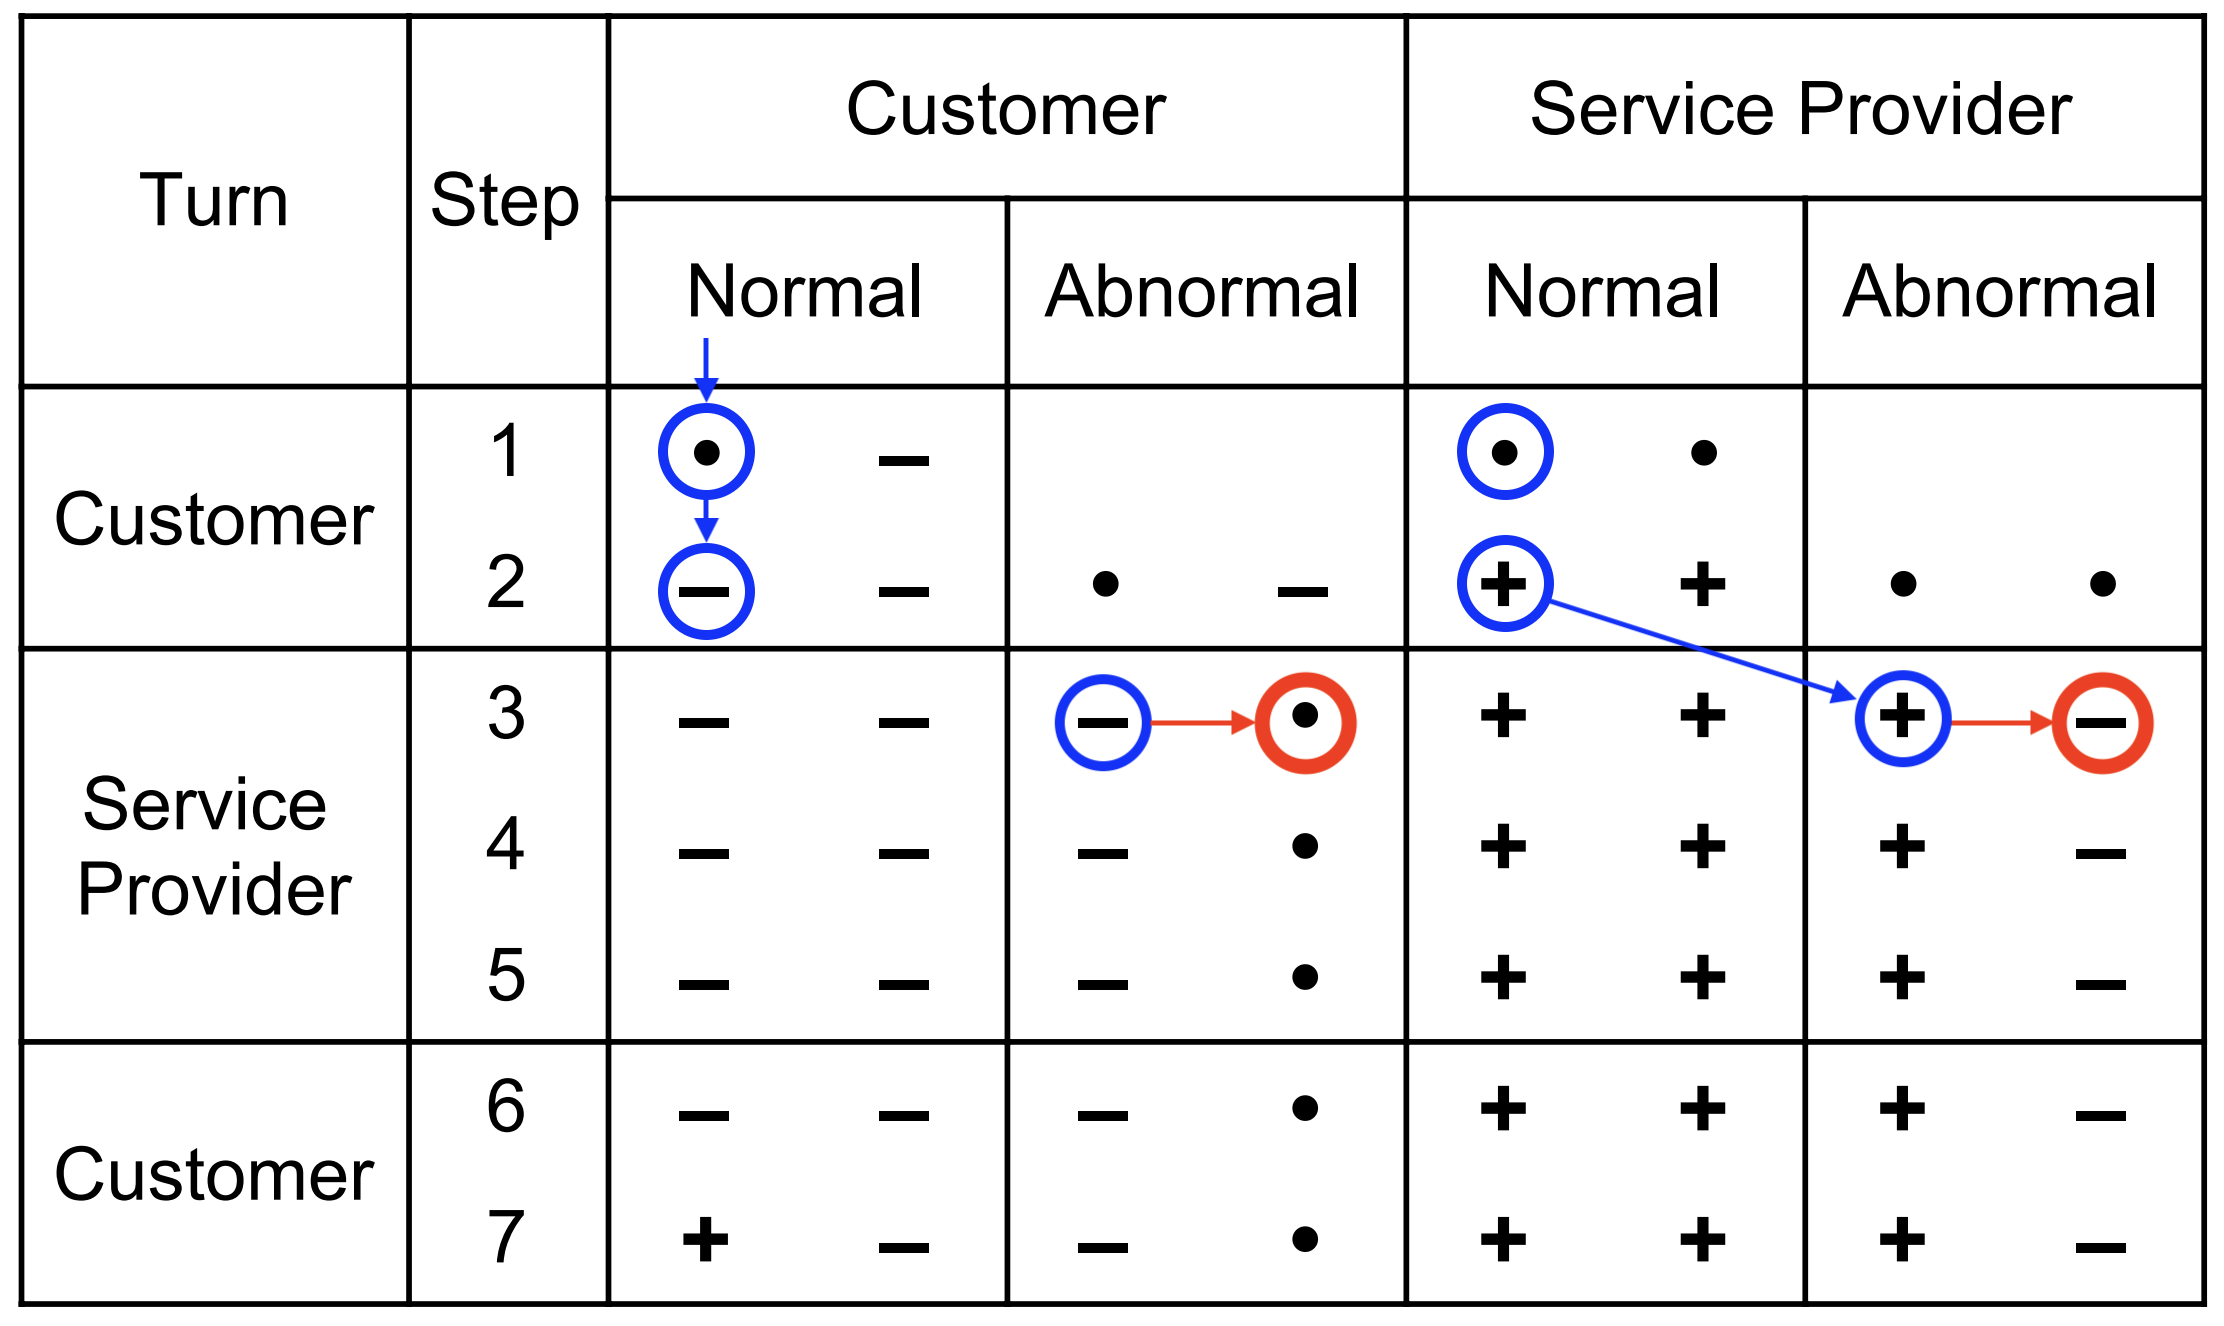
\includegraphics[width=9cm]{formal-misbehaviour-path.png}
\centering
\caption{Scenario of paths where the SP is misbehaving and the customer starts a dispute}
\label{fig:misbehaviour}
\end{figure}

Ultimately, the rational path for both parties is to follow the protocol as shown in the diagram below.

\begin{figure}[h!]
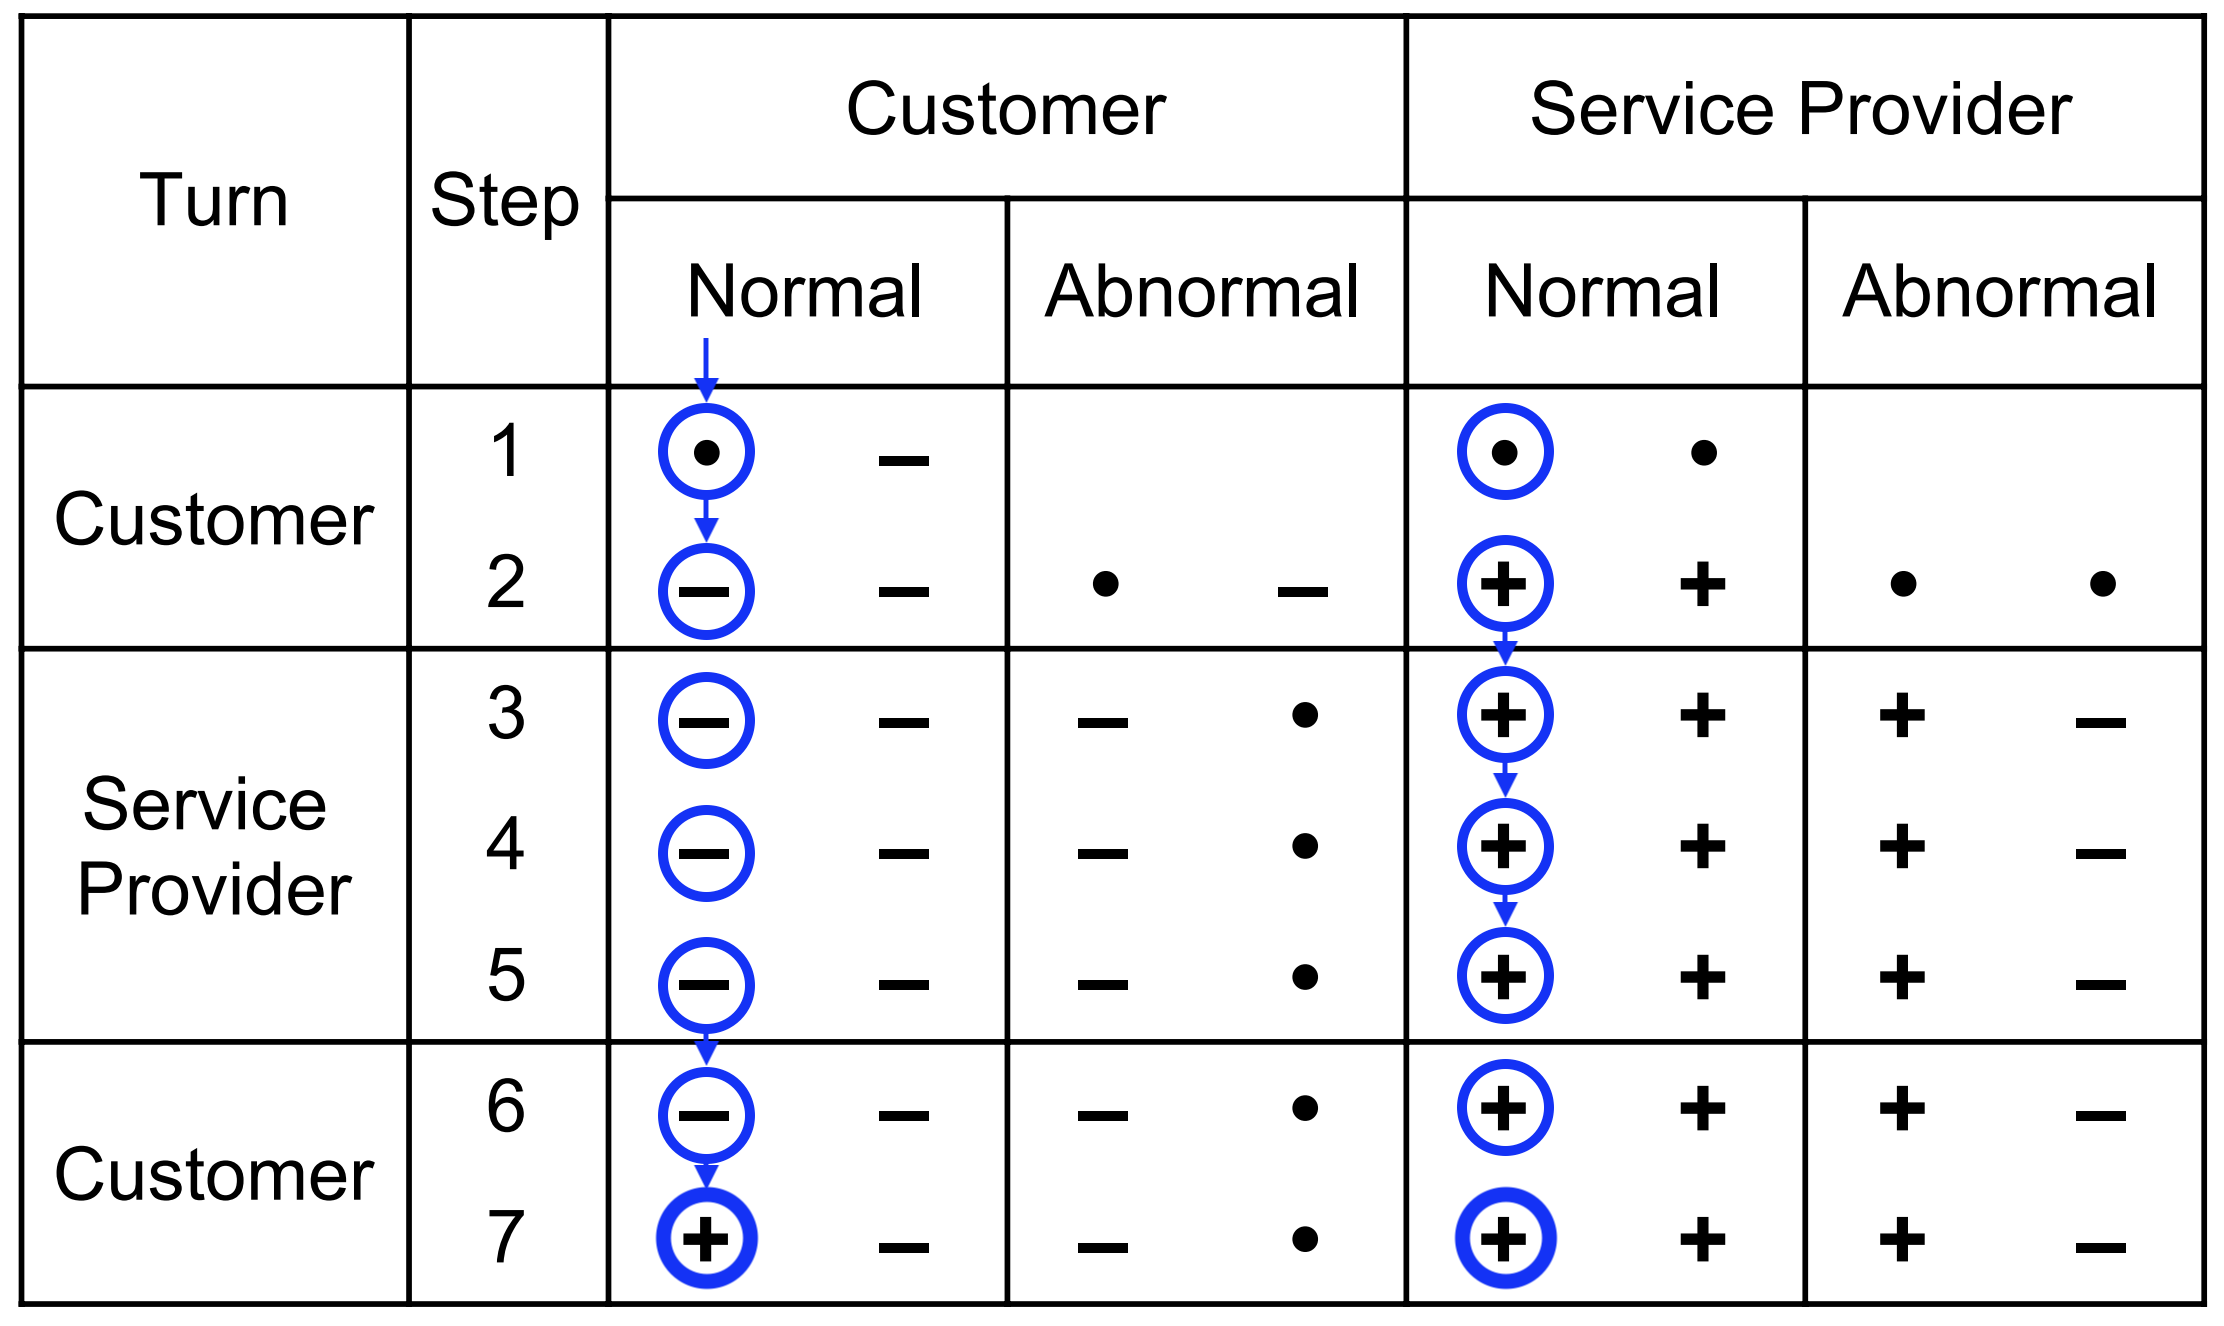
\includegraphics[width=9cm]{formal-rational-path.png}
\centering
\caption{The scenario of path where both the customer and  the SP are behaving correctly}
\label{fig:well-behaviour}
\end{figure}

%\subsection{Results}\label{results}

With the fairness definition stated in the equation and the assumptions stated in Section \ref{assumptions}, our analysis indicates that the protocol achieves fairness.



\section{Future work}
\label{sec:future-work}

\subsection{Justice}\label{justice}

Justice is the one biggest obstacle in achieving a system that complies with Web3 postulates~\cite{Web3Wiki71}.

The possible directions for mitigation of such issues are to either (1) replace justice with decentralized autonomous organizations (DAO) like proposed in Themis~\cite{meng2019themis} or Kleros~\cite{lesaege2018kleros}; or (2) make it infeasible to provide incorrect result.

The first approach is more feasible shortly. It would require creating a large pool of experts in a field, that in case of dispute, would receive all the proofs ($\mathrm{PoD}$, $\mathrm{PoP}$, as well as any other proofs significant to the case) that could be queried by the experts in zero-knowledge fashion, i.e., they could ask a limited number of questions to the proofs and getting yes/no answers. Keeping the case fully confidential. The experts would be incentivized to participate in the pool by the system of fees. Their honest behavior would be incentivized by the stake they would have to lock, and punishment they would get by judging incorrectly, where the ``correctly'' is determined by the quorum of votes.

The second approach is more philosophical and visionary. Suppose that the service we are undertaking is fully computable. Then, it would be possible by employing proofs of correctness of computations~\cite{ben2013snarks} to enforce that only correct computations (hence correct services) are accepted. To do so the whole service examination would have to be computable, which is hard to achieve in settings where physical materials (like blood) are examined. Concretely, the problem canes down to ``How to digitally represent blood''. If we could represent urine, blood, saliva, or any other physical material in binary format, and let the customer take a sample, discrete it, and send it to the SP by himself, then the whole chain of integrity could be ensured. Therefore, wrong service provision would be infeasible.


\subsection{Provable availability of the
result}\label{cryptographically-provable-availability-of-results}

Currently, the SP has to publish the result into a peer-to-peer content-addressable storage network, e.g., IPFS. The problem is that nothing prevents the SP from publishing the result, receiving the cid, publishing $\mathrm{PoP}$, and immediately after removing the result from the local storage. In case of dispute, the SP can upload the content again, proving its availability. The SP has no motivation to proceed with this kind of misbehavior, other than putting the customer in a disadvantaged position caused by the lost dispute. We see possible prevention of this misbehavior by the usage of Filecoin---an incentive layer on top of IPFS that guarantees the content availability via economic incentivisations~\cite{benetfilecoin}. With the help of Filecoin, the SP would be obligated to create a deal that guarantees the result availability until the deadline of the transaction. Moreover, since Filecoin is a blockchain by itself, it could play both roles of message board and storage network.

\subsection{Paying with cash}\label{paying-with-cash}

Without loss of generality, the payment can be made with cash. The customer can exchange the cash with SP together with delivering the package. The $\mathrm{PoD}$ would contain information that the transaction has been paid with cash; therefore, Steps 1 and 2 could be merged and realized in one step. In case of dispute, the payment disclosure would be included in $\mathrm{PoD}$.

\subsection{Anonymous delivery}\label{anonymous-delivery}

We assumed the customer to deliver the package to the SP personally or via a trusted person. However, the system could be extended to support an anonymous delivery system as proposed in Lelantos~\cite{altawy2017lelantos}.

\section{Conclusions}\label{sec:conclusion}
In this paper, we have proposed anonymity-preserving blockchain-based protocol for services provision. The protocol can be employed to provide services without collecting any personal information. The payment is handled by anonymous cryptocurrencies. Proof of delivery and proof of provision are published on the message board blockchain. The result is published on a content-addressable p2p network. The dispute can be settled by disclosing proof to justice. 
Using the definition~\ref{fairness} we showed that the protocol achieves fairness. Finally, we pinpointed further improvements like decentralized dispute resolution, provable availability of the result, paying with cash, and anonymous delivery via courier.

\bibliographystyle{IEEEtran}
% argument is your BibTeX string definitions and bibliography database(s)
\bibliography{bibliography}
%JS uporządkować bibliografię
\EOD

\end{document}

\setcounter{page}{0}
\newcommand{\floor}[1]{\left\lfloor #1 \right\rfloor}
\newcommand{\ceil}[1]{\left\lceil #1 \right\rceil}
